\chapter{Sistema de adquisición de datos DAQ}

  \section{Máquina de estados finitos (FSM)}

    \subsection{Introducción}

    Una máquina de estados finitos (FSM, por sus siglas en inglés) se utiliza para modelar un sistema que transita entre un número finito de estados internos, con transiciones que dependen del estado actual y de una entrada externa. A diferencia de un circuito secuencial convencional, las transiciones de estado de una FSM no siguen un patrón simple y repetitivo. La lógica de estado siguiente en una FSM generalmente se construye desde cero y a veces se conoce como lógica aleatoria. Esto contrasta con la lógica de estado siguiente en un circuito secuencial estándar, que suele estar compuesta principalmente por componentes estructurados, como incrementadores y desplazadores. En la práctica, la principal aplicación de una FSM es funcionar como el controlador de un gran sistema digital, examinando los comandos externos y el estado del sistema, y activando las señales de control adecuadas para gestionar la operación de un \textit{data path}, que suele estar compuesta por componentes secuenciales convencionales. Esto se conoce como FSMD (máquina de estados finitos con data path) del cual se tratará en una sección posterior.

    \subsection{Tipos de máquinas de estado}

    El diagrama de bloques básico de una FSM es similar al de un circuito secuencial regular y se muestra en la Figura \ref{fig:fsm_diagram}. Consta de un registro de estado, lógica de próximo estado y lógica de salida. Una FSM se denomina \textit{máquina Moore} si la salida depende únicamente del estado, y se denomina \textit{máquina Mealy} si la salida depende tanto del estado como de la entrada externa. En una FSM compleja, pueden coexistir ambos tipos de salida, y en ese caso, se dice que la FSM contiene una salida Moore y una salida Mealy. Aunque las salidas Moore y Mealy son similares, no son idénticas. Entender sus diferencias sutiles es fundamental para el diseño de controladores.

    \begin{figure}[h!]
      \centering
      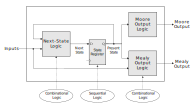
\includegraphics[width=0.95\textwidth]{fsm_diagram}
      \caption{Diagrama a bloques de una FSM con salidas Moore y Mealy.}
      \label{fig:fsm_diagram}
    \end{figure}

    \subsection{Moore vs Mealy}

    Las máquinas de estados de tipo Moore son preferidas en la industria porque las salidas disponen de un ciclo completo para estabilizarse a través de la lógica combinacional, lo que facilita el cumplimiento de los tiempos de ciclo requeridos. Por otro lado, las salidas de tipo Mealy permiten que una entrada se procese después de que el ciclo ha comenzado, y dicha entrada debe atravesar la lógica combinacional y cumplir con el tiempo de preparación para la salida Mealy. Si el diseño requiere absolutamente que una entrada llegue al chip después del flanco activo del reloj, pase por la lógica y se refleje en la salida dentro de un solo ciclo, esos diseños suelen emplear una salida Mealy.

    Usando un juego de palabras en inglés, se dice que ``Moore is Less'', lo que hace referencia a que las máquinas de estados de Moore dependen únicamente del estado actual, mientras que las máquinas de estados de Mealy dependen tanto del estado actual como de una o más entradas. 

    En general, se evitan los diseños de FSM de Mealy a menos que sean absolutamente necesarios.

    \subsection{Representación de FSM}

    Una FSM generalmente se describe mediante un diagrama de estados abstracto o un diagrama ASM (diagrama de máquina de estados algorítmica), ambos capturando la entrada, salida, estados y transiciones de la FSM en una representación gráfica. Ambas representaciones contienen la misma información. El diagrama de estados es más compacto y adecuado para aplicaciones simples, mientras que el diagrama ASM, que se asemeja a un diagrama de flujo, es más descriptivo y útil para aplicaciones con condiciones de transición y acciones complejas.

    \textbf{Diagrama de estados}: Un diagrama de estados se compone de \textit{nodos}, que representan estados y se dibujan como círculos, y \textit{arcos de transición} anotados. Un solo nodo y sus arcos de transición se muestran en la Figura \ref{fig:node_asm_diagram}(\subref{fig:node}). Cada arco de transición está asociado con una expresión lógica expresada en términos de señales de entrada, que representa una condición específica. El arco se toma cuando la expresión correspondiente se evalúa como verdadera.

    Los valores de salida Moore se ubican dentro del círculo, ya que dependen exclusivamente del estado actual. Los valores de salida Mealy, por su parte, se asocian con las condiciones de los arcos de transición, dado que dependen tanto del estado actual como de la entrada externa. Para mantener el diagrama más claro y ordenado, solo se muestran los valores de salida que están activos. En caso contrario, la señal de salida toma su valor predeterminado (es decir, inactivo).

    En la Figura \ref{fig:fsm_asm_example}(\subref{fig:fsm_example}) se muestra un diagrama de estados representativo. La FSM tiene tres estados, dos señales de entrada externas ($a$ y $b$), una señal de salida Moore ($y_{1}$) y una señal de salida Mealy ($y_{0}$). La señal $y_{1}$ se activa cuando la FSM se encuentra en los estados $S_{0}$ o $S_{1}$. Por otro lado, la señal $y_{0}$ se activa cuando la FSM está en el estado $S_{0}$ y las señales $a$ y $b$ están en 1 respectivamente.

    \textbf{Diagrama ASM}: Un diagrama ASM está compuesto por una red de bloques ASM. Un \textit{bloque ASM} incluye una \textit{caja de estado} y, de manera opcional, una red de \textit{cajas de decisión} y \textit{cajas de salida condicional}. En la Figura \ref{fig:fsm_asm_example}(\subref{fig:asm}) se muestra un bloque ASM representativo.

    Una caja de estado representa un estado en una FSM, y dentro de ella se enumeran los valores de salida de Moore que están activos. Es importante destacar que esta caja tiene solo un camino de salida. Una caja de decisión evalúa la condición de entrada y determina cuál camino de salida seguir. Esta caja tiene dos caminos de salida, etiquetados como T y F, que corresponden a los valores verdadero y falso de la condición. Una caja de salida condicional enumera los valores de salida Mealy que están activos y generalmente se coloca después de una caja de decisión. Esta caja indica que la señal de salida listada solo puede activarse cuando se cumple la condición correspondiente en la caja de decisión.

    Un diagrama de estados puede convertirse fácilmente en un diagrama ASM, y viceversa. El diagrama ASM correspondiente al diagrama de estado FSM anterior se muestra en la Figura \ref{fig:fsm_asm_example}(\subref{fig:asm_example}).

    \begin{figure}[!h]
        \centering
        \subfloat[Nodo\label{fig:node}]{{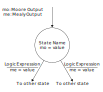
\includegraphics[width=0.4\textwidth]{node_diagram} }}
        \subfloat[Bloque ASM\label{fig:asm}]{{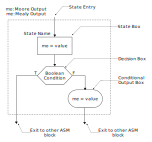
\includegraphics[width=0.55\textwidth]{asm_diagram} }}
        \caption{Simbolo de un estado.}
        \label{fig:node_asm_diagram}
    \end{figure}

    \begin{figure}[!h]
        \centering
        \subfloat[Diagrama de estados\label{fig:fsm_example}]{{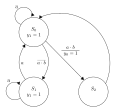
\includegraphics[width=0.45\textwidth]{fsm_example} }}
        \subfloat[Diagrama ASM\label{fig:asm_example}]{{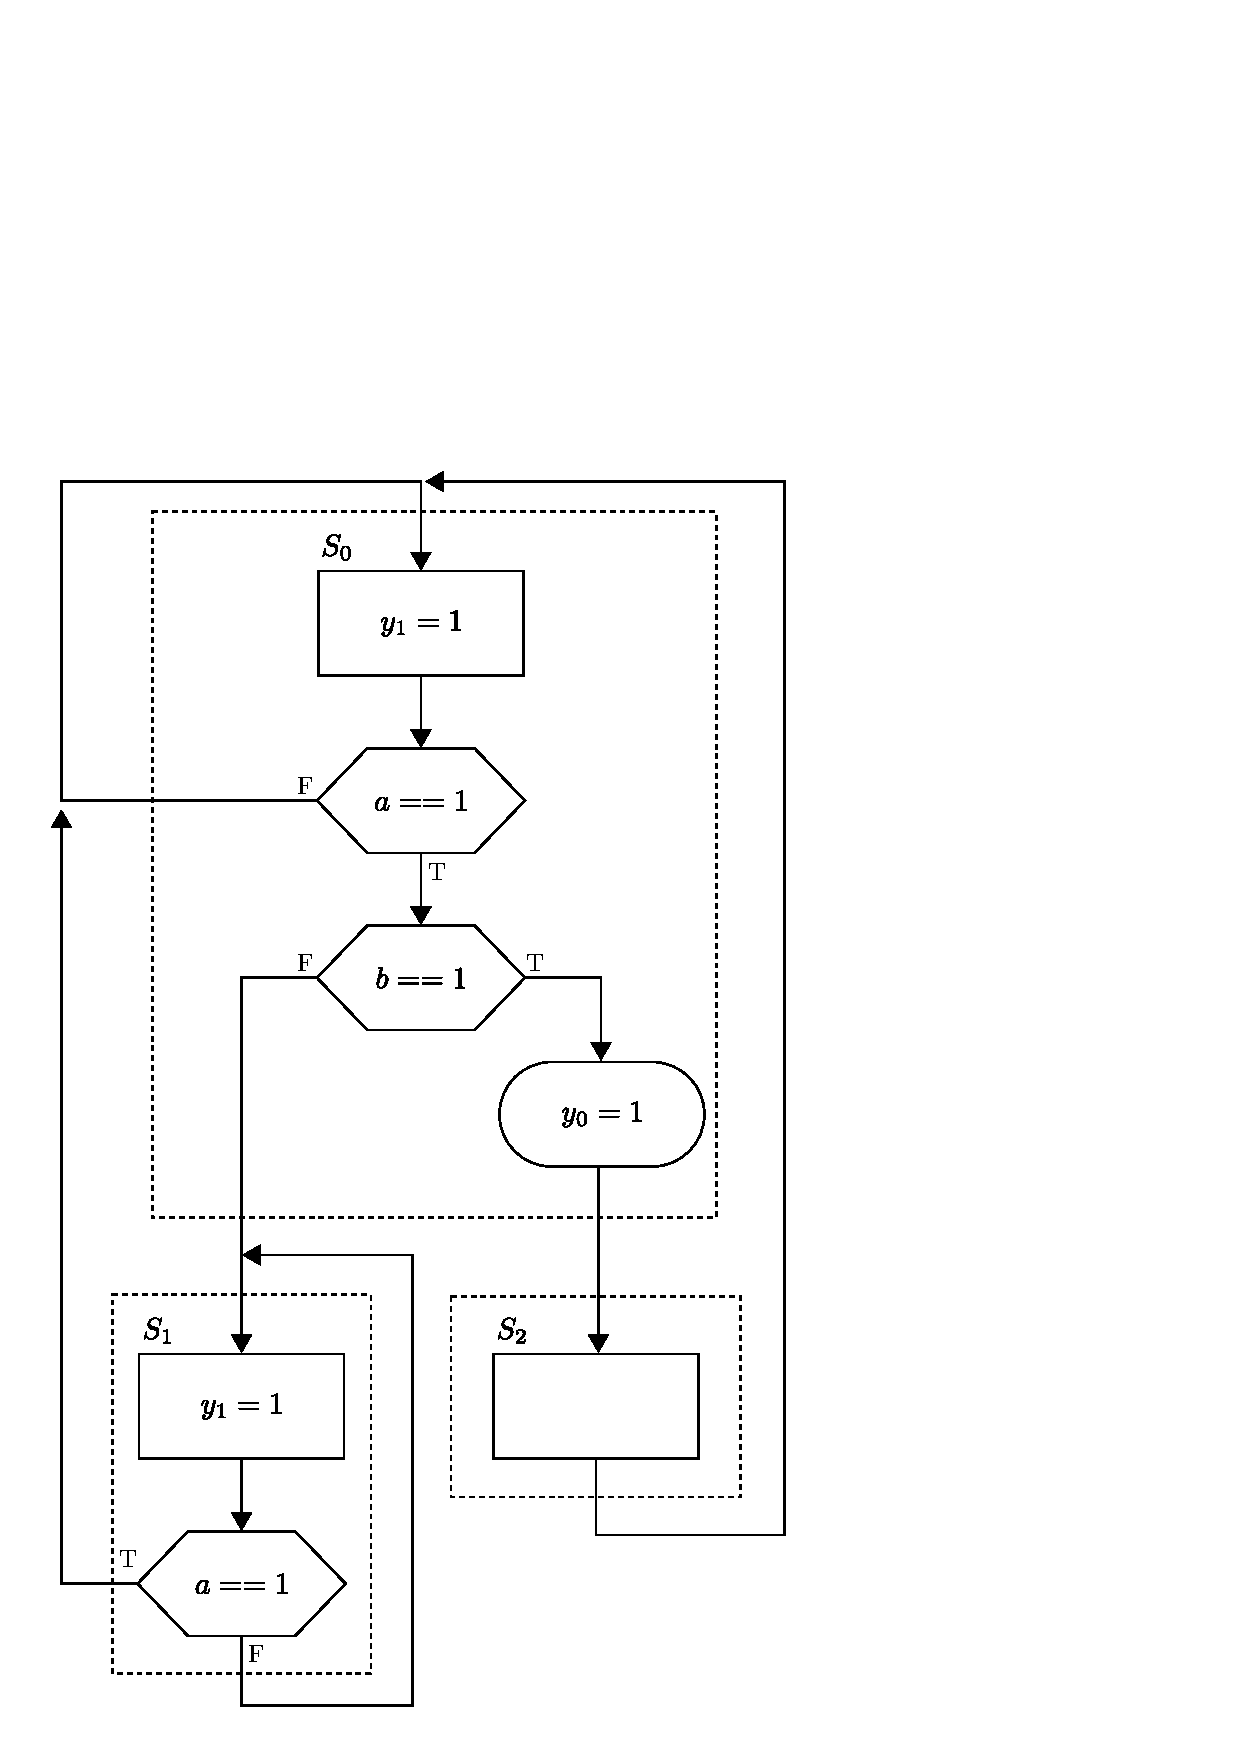
\includegraphics[width=0.45\textwidth]{asm_example} }}
        \caption{Ejemplo de una FSM.}
        \label{fig:fsm_asm_example}
    \end{figure}


    \subsection{FSM con data path (FSMD)}

    Una FSMD (máquina de estados finitos con data path) combina una FSM y circuitos secuenciales regulares. La FSM, que a veces se conoce como \textit{control path}, examina los comandos externos y el estado, y genera señales de control para especificar la operación de los circuitos secuenciales regulares, que en conjunto se conocen como \textit{data path}. La FSMD se utiliza para implementar sistemas descritos por la \textit{metodología RT} (register transfer), en la cual las operaciones se especifican como manipulación y transferencia de datos entre un conjunto de registros.

    \subsection{Operación RT simple}

    Una operación RT especifica la manipulación y transferencia de datos para un único registro de destino. Se representa mediante la notación

    \begin{equation}
      r_{\text{dest}} \leftarrow f( r_{\text{src1}}, r_{\text{src2}}, \ldots, r_{\text{srcn}})
    \end{equation}
    donde $r_{\text{dest}}$ es el registro de destino, $r_{\text{src1}}$, $r_{\text{src2}}$ y $r_{\text{srcn}}$ son los registros de origen, y $f(\cdot)$ especifica la operación a realizar. La notación indica que el contenido de los registros de origen se alimenta a la función $f(\cdot)$, que se realiza mediante un circuito combinacional, y el resultado se pasa a la entrada del registro de destino y se almacena en el registro de destino en el siguiente flanco ascendente del reloj. 

    A continuación se presentan varias operaciones RT representativas:

    \begin{itemize}
      \item $r1 \leftarrow 0$. Se almacena una constante 0 en el registro $r1$.
      \item $r1 \leftarrow r1$. El contenido del registro $r1$ se escribe de nuevo sobre sí mismo.
      \item $r2 \leftarrow r2 >> 3$. El registro $r2$ se desplaza tres posiciones a la derecha y luego se escribe de nuevo sobre sí mismo.
      \item $r2 \leftarrow r1$. El contenido del registro $r1$ se transfiere al registro $r2$.
      \item $i \leftarrow i + 1$. El contenido del registro $i$ se incrementa en 1 y el resultado se escribe sobre sí mismo.
      \item $d \leftarrow s1 + s2 + s3$. La suma de los registros $s1$, $s2$ y $s3$ se escribe en el registro $d$.
      \item $y \leftarrow a \cdot a$. El cuadrado de $a$ se escribe en el registro $y$.
    \end{itemize}

     Una operación RT simple puede implementarse construyendo un circuito combinacional para la función $f(\cdot)$ y conectando la entrada y la salida de los registros. Por ejemplo, considere la operación $a \leftarrow a - b + 1$. La función $f(\cdot)$ implica un restador y un incrementador. El diagrama de bloques se muestra en la Figura \ref{fig:rt_figure}(\subref{fig:rt_example}). Para mayor claridad, utilizamos los sufijos ``\_next'' y ``\_reg'' para representar la entrada y la salida de un registro. Nótese que una operación RT está sincronizada por un reloj incorporado. El resultado de la función $f(\cdot)$ no se almacena en el registro de destino hasta el siguiente flanco ascendente del reloj. El diagrama de tiempo de la operación RT anterior se muestra en la Figura \ref{fig:rt_figure}(\subref{fig:rt_example_timing}).

    \begin{figure}[!h]
        \centering
        \subfloat[Diagrama de bloques de ejemplo RT\label{fig:rt_example}]{{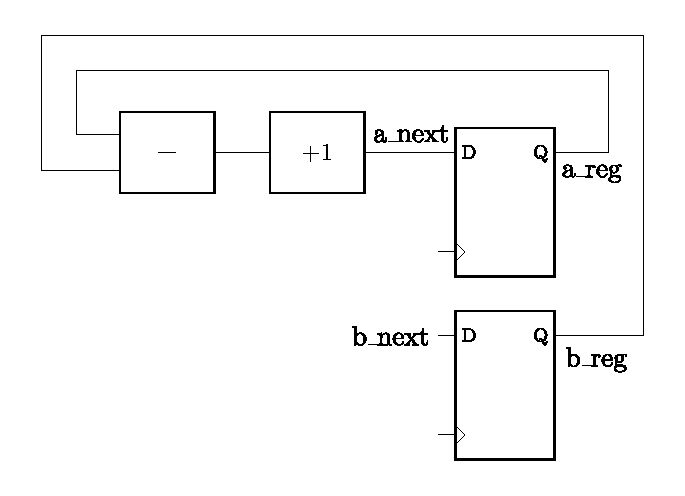
\includegraphics[width=0.6\textwidth]{rt_example} }}\\
        \subfloat[Diagrama de tiempo de ejemplo RT\label{fig:rt_example_timing}]{{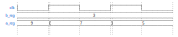
\includegraphics[width=0.95\textwidth]{rt_example_timing} }}
        \caption{Diagramas de bloques y de tiempo de una operación RT.}
        \label{fig:rt_figure}
    \end{figure}

     \subsection{Diagrama ASMD}

      Un circuito basado en la metodología de transferencia de registros (RT) especifica qué operaciones RT deben ejecutarse en cada paso. Dado que una operación RT se realiza en un ciclo de reloj, su temporización es similar a la transición de estado de una FSM. Por ello, una FSM es la opción natural para especificar la secuenciación de un algoritmo RT. 

      Se extiende el diagrama ASM para incorporar operaciones RT y se denomina \textit{diagrama ASMD} (ASM con data path). Las operaciones RT se tratan como otro tipo de actividad y pueden ubicarse en los mismos lugares donde se utilizan las señales de salida.

    \begin{figure}[!h]
        \centering
        \subfloat[Segmento ASMD\label{fig:asmd_segment}]{{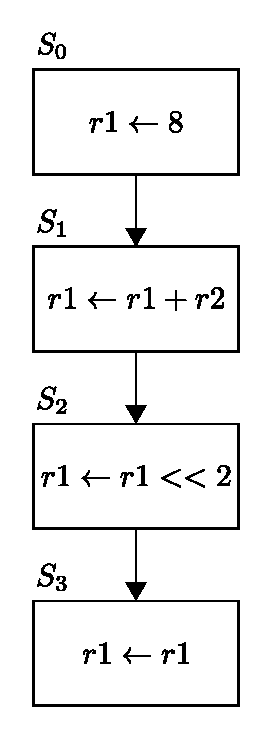
\includegraphics[width=0.16\textwidth]{asmd_segment} }}
        \subfloat[Diagrama de bloques\label{fig:asmd_segment_diagram}]{{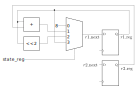
\includegraphics[width=0.7\textwidth]{asmd_segment_diagram} }}
        \caption{Realización de segmento ASMD.}
        \label{fig:asmd_figure}
    \end{figure}

    Un segmento de un diagrama ASMD se muestra en la Figura \ref{fig:asmd_figure}(\subref{fig:asmd_segment}). Este segmento incluye un registro de destino, $r1$, que se inicializa con el valor 8, se suma con el contenido del registro $r2$, y luego se desplaza dos posiciones a la izquierda. Es importante señalar que el registro $r1$ debe especificarse en cada estado. Cuando $r1$ no se modifica, se debe usar la operación $r1 \leftarrow r1$ para mantener su contenido actual, como en el estado $S_{3}$. En algunos diagramas, se asume que $r1 \leftarrow r1$ es la operación RT predeterminada para el registro $r1$ y, por lo tanto, no se incluye en el diagrama ASMD. Implementar las operaciones RT de un diagrama ASMD requiere un circuito de multiplexación para dirigir el siguiente valor deseado al registro de destino. Por ejemplo, el segmento anterior puede implementarse mediante un multiplexor de 4 a 1, como se muestra en la Figura \ref{fig:asmd_figure}(\subref{fig:asmd_segment_diagram}). El estado actual de la FSM (es decir, la salida del registro de estado) controla la señal de selección del multiplexor, seleccionando así el resultado de la operación RT deseada.

    Una operación RT también puede especificarse en una caja de salida condicional, como se muestra con el registro $r2$ en la Figura \ref{fig:asmd_rt_figure}(\subref{fig:asmd_rt_operation_diagram}). Dependiendo de la condición $a>b$, la FSMD ejecutará $r2 \leftarrow r2+a$ o $r2 \leftarrow r2+b$. Es importante señalar que todas las operaciones dentro de un bloque ASMD se realizan en paralelo. Para implementar esto, se necesitan realizar las operaciones $a>b$, $r2+a$ y $r2+b$, y utilizar un multiplexor para dirigir el valor deseado hacia $r2$. El diagrama de bloques correspondiente se muestra en la Figura \ref{fig:asmd_rt_figure}(\subref{fig:asmd_rt_operation}).

    \begin{figure}[!h]
        \centering
        \subfloat[Diagrama de bloques\label{fig:asmd_rt_operation_diagram}]{{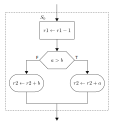
\includegraphics[width=0.4\textwidth]{asmd_rt_operation_diagram} }}
        \subfloat[Bloque ASM\label{fig:asmd_rt_operation}]{{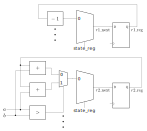
\includegraphics[width=0.55\textwidth]{asmd_rt_operation} }}
        \caption{Realización de una operación RT en una caja de salida condicional.}
        \label{fig:asmd_rt_figure}
    \end{figure}

    \subsection{Caja de decisión con registro}

    La apariencia de un diagrama ASMD es similar a la de un diagrama de flujo convencional. La principal diferencia radica en que la operación RT en un diagrama ASMD está controlada por una señal de reloj interna, y el registro de destino se actualiza \text{cuando el FSMD sale del bloque ASMD actual}, pero no dentro del bloque. La operación $r + r-1$ en realidad significa que:

    \begin{itemize}
      \item \texttt{r\_next = r\_reg - 1}
      \item \texttt{r\_reg = r\_next} en el flanco ascendente del reloj (es decir, cuando el FSMD sale del bloque actual).
    \end{itemize}

    Este almacenamiento retrasado puede introducir errores sutiles cuando se utiliza un registro en una caja de decisión. Considere el segmento FSMD en la Figura \ref{fig:asm_affected_delay}(\subref{fig:asm_affected_delay_old}). El registro $r$ se decrementa en la caja de estado y se utiliza en la caja de decisión. Dado que el registro $r$ no se actualiza hasta que el FSMD sale del bloque, el contenido antiguo de $r$ se utiliza para la comparación en la caja de decisión. Si se desea utilizar el nuevo valor de $r$, se debe usar la salida de la lógica combinacional (es decir, $r\_$next) en la caja de decisión (es decir, reemplazar la expresión $r == 0$ con $r\_$next $==0$), como se muestra en la Figura \ref{fig:asm_affected_delay}(\subref{fig:asm_affected_delay_new}).

    \begin{figure}[!h]
        \centering
        \subfloat[Utilizar el valor antiguo de $r$\label{fig:asm_affected_delay_old}]{{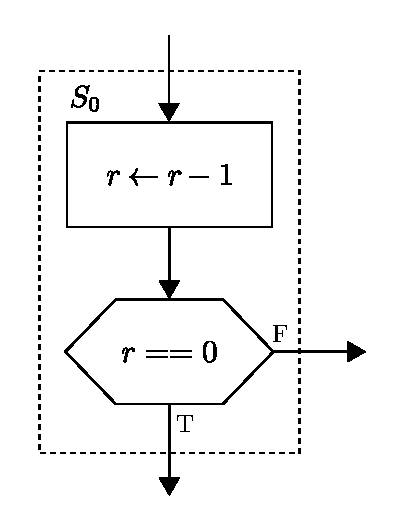
\includegraphics[width=0.35\textwidth]{asm_affected_delay_old} }}
        \subfloat[Utilizar el nuevo valor de $r$\label{fig:asm_affected_delay_new}]{{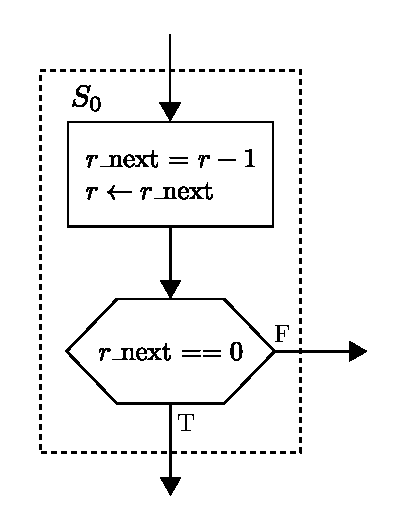
\includegraphics[width=0.35\textwidth]{asm_affected_delay_new} }}
        \caption{Bloque ASM afectado por un almacenamiento retrasado.}
        \label{fig:asm_affected_delay}
    \end{figure}

    \subsection{Diagrama de bloques de una FSMD}

    El diagrama de bloques conceptual de una FSMD se divide en \textit{data path} y en \textit{control path}, como se muestra en la Figura \ref{fig:fsmd_block_diagram}. El \textit{data path} se encarga de ejecutar las operaciones RT necesarias. Consiste en:

    \begin{itemize}
      \item \textit{Data registers}: almacenan los resultados intermedios de los cálculos.
      \item \textit{Functional units}: realizan las funciones especificadas por las operaciones RT.
      \item \textit{Routing network}: dirige los datos entre los registros de almacenamiento y las unidades funcionales.
    \end{itemize}

    El \textit{data path} sigue la \textbf{señal de control} (Control Signal) para llevar a cabo las operaciones RT deseadas y genera la señal de \textbf{estado interno} (Internal Status).

    \begin{figure}[!h]
      \centering
      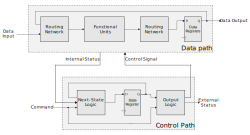
\includegraphics[width=0.95\textwidth]{fsmd_block_diagram}
      \caption{Diagrama de bloques de una FSMD.}
      \label{fig:fsmd_block_diagram}
    \end{figure}

    El \textit{control path} es una FSM. Al igual que cualquier FSM convencional, contiene un registro de estado, lógica de próximo estado y lógica de salida. Utiliza la señal de \textbf{comando} (Command) externa y la señal de \textbf{estado interno} (Internal Status) del \textit{data path} como entradas, y genera la \textbf{señal de control} (Control Signal) que regula la operación del \textit{data path}. Además, la FSM genera una señal de \textbf{estado externa} (External Status) para indicar el estado de la operación del FSMD.

    Es importante destacar que, aunque un FSMD está compuesta por dos tipos de circuitos secuenciales, ambos circuitos son controlados por el mismo reloj, lo que mantiene al FSMD como un sistema síncrono.

  \section{Visión general de la comunicación serial}

    Con frecuencia, un sistema necesita comunicarse con otro que no reside en el mismo dispositivo. Para reducir el número de pines de I/O y el cableado externo, los dos sistemas pueden transferir datos a través de una única línea serial, bit a bit. El sistema transmisor realiza la conversión de paralelo a serie y, a continuación, envía los datos serie a través de una única línea. El sistema receptor realiza la conversión serie a paralelo y restaura los datos paralelos originales.

    La comunicación serial puede utilizarse tanto para transferir datos a alta velocidad como a baja velocidad. En una interfaz de alta velocidad, como USB y gigabit Ethernet, la velocidad de transmisión de datos puede alcanzar varios cientos de millones de bits por segundo o más. 

    En una interfaz de baja velocidad, la velocidad de transmisión de datos oscila entre varios miles y varios cientos de miles de bits por segundo. Es adecuada para la mayoría de los periféricos de I/O generales y para tareas de adquisición y control de datos. Dado que la velocidad de datos es mucho más lenta que la velocidad de reloj de una FPGA, estos esquemas pueden ser realizados por los elementos lógicos genéricos de una FPGA. A continuación se discuten los esquemas UART y SPI.

	\section{Controlador UART}

    La comunicación serial utiliza una única línea de datos para intercambiar información entre dos sistemas. El sistema transmisor convierte los datos paralelos en un flujo serie y el sistema receptor vuelve a ensamblar los datos serie en su formato paralelo original. El esquema más utilizado es el UART, (Universal Asynchronous Receiver and Transmitter) o receptor y transmisor asíncrono universal en español.

    \subsection{Visión general}

    Un controlador UART básico incluye un transmisor y un receptor. El transmisor es un registro de corrimiento especial que carga datos en paralelo y luego los desplaza bit a bit a una velocidad específica. El receptor, por su parte, desplaza los datos bit a bit y los vuelve a ensamblar. La línea serial es 1 cuando está inactiva. La transmisión comienza con un bit de inicio, que es 0, seguido de bits de datos y un bit de paridad opcional, y termina con bits de parada, que son 1. El número de bits de datos puede ser 6, 7 u 8. El bit de paridad opcional se utiliza para la detección de errores. Para paridad impar, se pone a 0 cuando los bits de datos tienen un número impar de 1's. Para paridad par, se pone a 0 cuando los bits de datos tienen un número par de 1's. El número de bits de parada puede ser 1, 1,5 ó 2. En la Figura \ref{fig:uart_transmission} se muestra la transmisión con ocho bits de datos, sin paridad y un bit de parada. Observe que el LSB de la palabra de datos se transmite primero.

    \begin{figure}[hbtp]
      \centering
      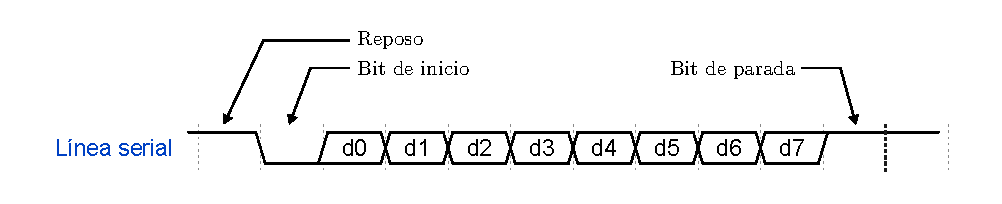
\includegraphics[width=0.95\textwidth]{uart_transmission}
      \caption{Diagrama de la transmisión de un byte serial con UART.}
      \label{fig:uart_transmission}
    \end{figure}

    A través de la línea serial no se transmite información de reloj. Antes de iniciar la transmisión, el transmisor y el receptor deben acordar de antemano una serie de parámetros, que incluyen la velocidad en baudios (es decir, el número de bits por segundo), el número de bits de datos y bits de parada, y el uso del bit de paridad. Con los parámetros predeterminados, el receptor utiliza un esquema de sobremuestreo para recuperar los bits de datos. Las velocidades en baudios más utilizadas son 9,600 y 19,200 baudios.

    \subsection{Procedimiento de sobremuestreo} \label{sec:sobremuestreo}

    La velocidad de muestreo más utilizada es 16 veces la velocidad en baudios, lo que significa que cada bit serie se muestrea 16 veces. Para un enlace de comunicación con N bits de datos y M bits de parada, el esquema de sobremuestreo funciona de la siguiente manera:
    
    \begin{enumerate}
      \item Espera hasta que la señal entrante se convierta en 0, el comienzo del bit de inicio, y luego comienza a contar los pulsos de muestreo.
      \item Cuando el contador llegue a 7, la señal entrante alcanzará el punto medio del bit de inicio. Limpia el contador a 0 y reinícialo.
      \item Cuando el contador llegue a 15, la señal entrante habrá avanzado un bit y alcanzará el punto medio del primer bit de datos. Obtén su valor, desplázalo a un registro y reinicia el contador.
      \item Repite el paso 3 N–1 veces más para obtener los bits de datos restantes.
      \item Si se utiliza el bit de paridad opcional, repite el paso 3 una vez para obtener el bit de paridad.
      \item Repite el paso 3 M veces más para obtener los bits de parada.
    \end{enumerate}

    El esquema de sobremuestreo realiza básicamente la función de una señal de reloj. En lugar de utilizar el flanco ascendente para indicar cuándo es válida la señal de entrada, utiliza los pulsos de muestreo para estimar el punto medio de cada bit. Aunque el receptor no tiene información sobre el momento exacto de inicio del bit, la estimación puede estar desviada como máximo en $1/16$. Las siguientes recuperaciones de bits de datos también se desvían como máximo de $1/16$ del punto medio. Debido al sobremuestreo, la velocidad en baudios sólo puede ser una pequeña fracción de la velocidad de reloj del sistema, por lo que este esquema no es apropiado para una velocidad de datos alta.


    \subsection{Diseño conceptual}

      El diagrama de alto nivel de un sistema UART se muestra en la Figura \ref{fig:uart_diagram}. Consiste en tres componentes principales. El generador de la tasa de baudios genera una señal de sobremuestreo. El receptor realiza la conversión de serie a paralelo y el transmisor realiza la conversión de paralelo a serie. El código completo integrando los tres componentes se muestra en el Código \ref{cod:uart_ip}.

    \begin{figure}[h!]
      \centering
      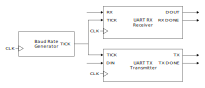
\includegraphics[width=0.8\textwidth]{uart_diagram}
      \caption{Diagrama de bloques de una controlador UART completo.}
      \label{fig:uart_diagram}
    \end{figure}

    \subsection{Generador de la tasa de baudios}

    El generador de la tasa de baudios genera una señal de muestreo cuya frecuencia es exactamente 16 veces la tasa de baudios designada para el UART. Para evitar la creación de un nuevo dominio de reloj y violar el principio de diseño síncrono, la señal de muestreo debe funcionar como pulsos de habilitación en lugar de la señal de reloj para el receptor UART.

    El generador de la tasa de baudios es un contador programable y el código HDL se muestra en el Código \ref{cod:baud_gen}. El código es un contador mod$-m$ parametrizado que se reinicia cada vez que el contador llega a un valor determinado. Por ejemplo para una tasa de 19,200 baudios, la tasa de muestreo tiene que ser de 307,200 (es decir, 19,200 $\times$ 16) pulsos por segundo. Dada una frecuencia del reloj de sistema de 50 MHz, el generador de la tasa de baudios necesita un contador mod-163, $\left( \frac{50 \times 10^{6}}{19200 \times 16} \right)$, en el cual se genera un pulso de ciclo de reloj cada 163 ciclos de reloj del sistema.

    \subsection{Receptor UART}

    El receptor UART obtiene el byte de datos de la línea serial mediante sobremuestreo. Utiliza la señal del generador de la tasa de baudios para estimar los puntos medios de los bits transmitidos y, a continuación, los recupera en esos puntos de manera precisa.
    
    La operación general de recepción se puede describir mediante un diagrama ASMD, como se muestra en la Figura \ref{fig:asmd_uart_rx}. Para permitir futuras modificaciones, se utilizan dos parámetros en la descripción. El parámetro D\_BIT indica el número de bits de datos, mientras que SB\_TICK representa el número de "ticks" necesarios para los bits de parada, que son 16, 24 y 32 para 1, 1.5 y 2 bits de parada, respectivamente. En este diseño, a D\_BIT y SB\_TICK se les asignaron los valores 8 y 16.

    \begin{figure}[hbtp]
      \centering
      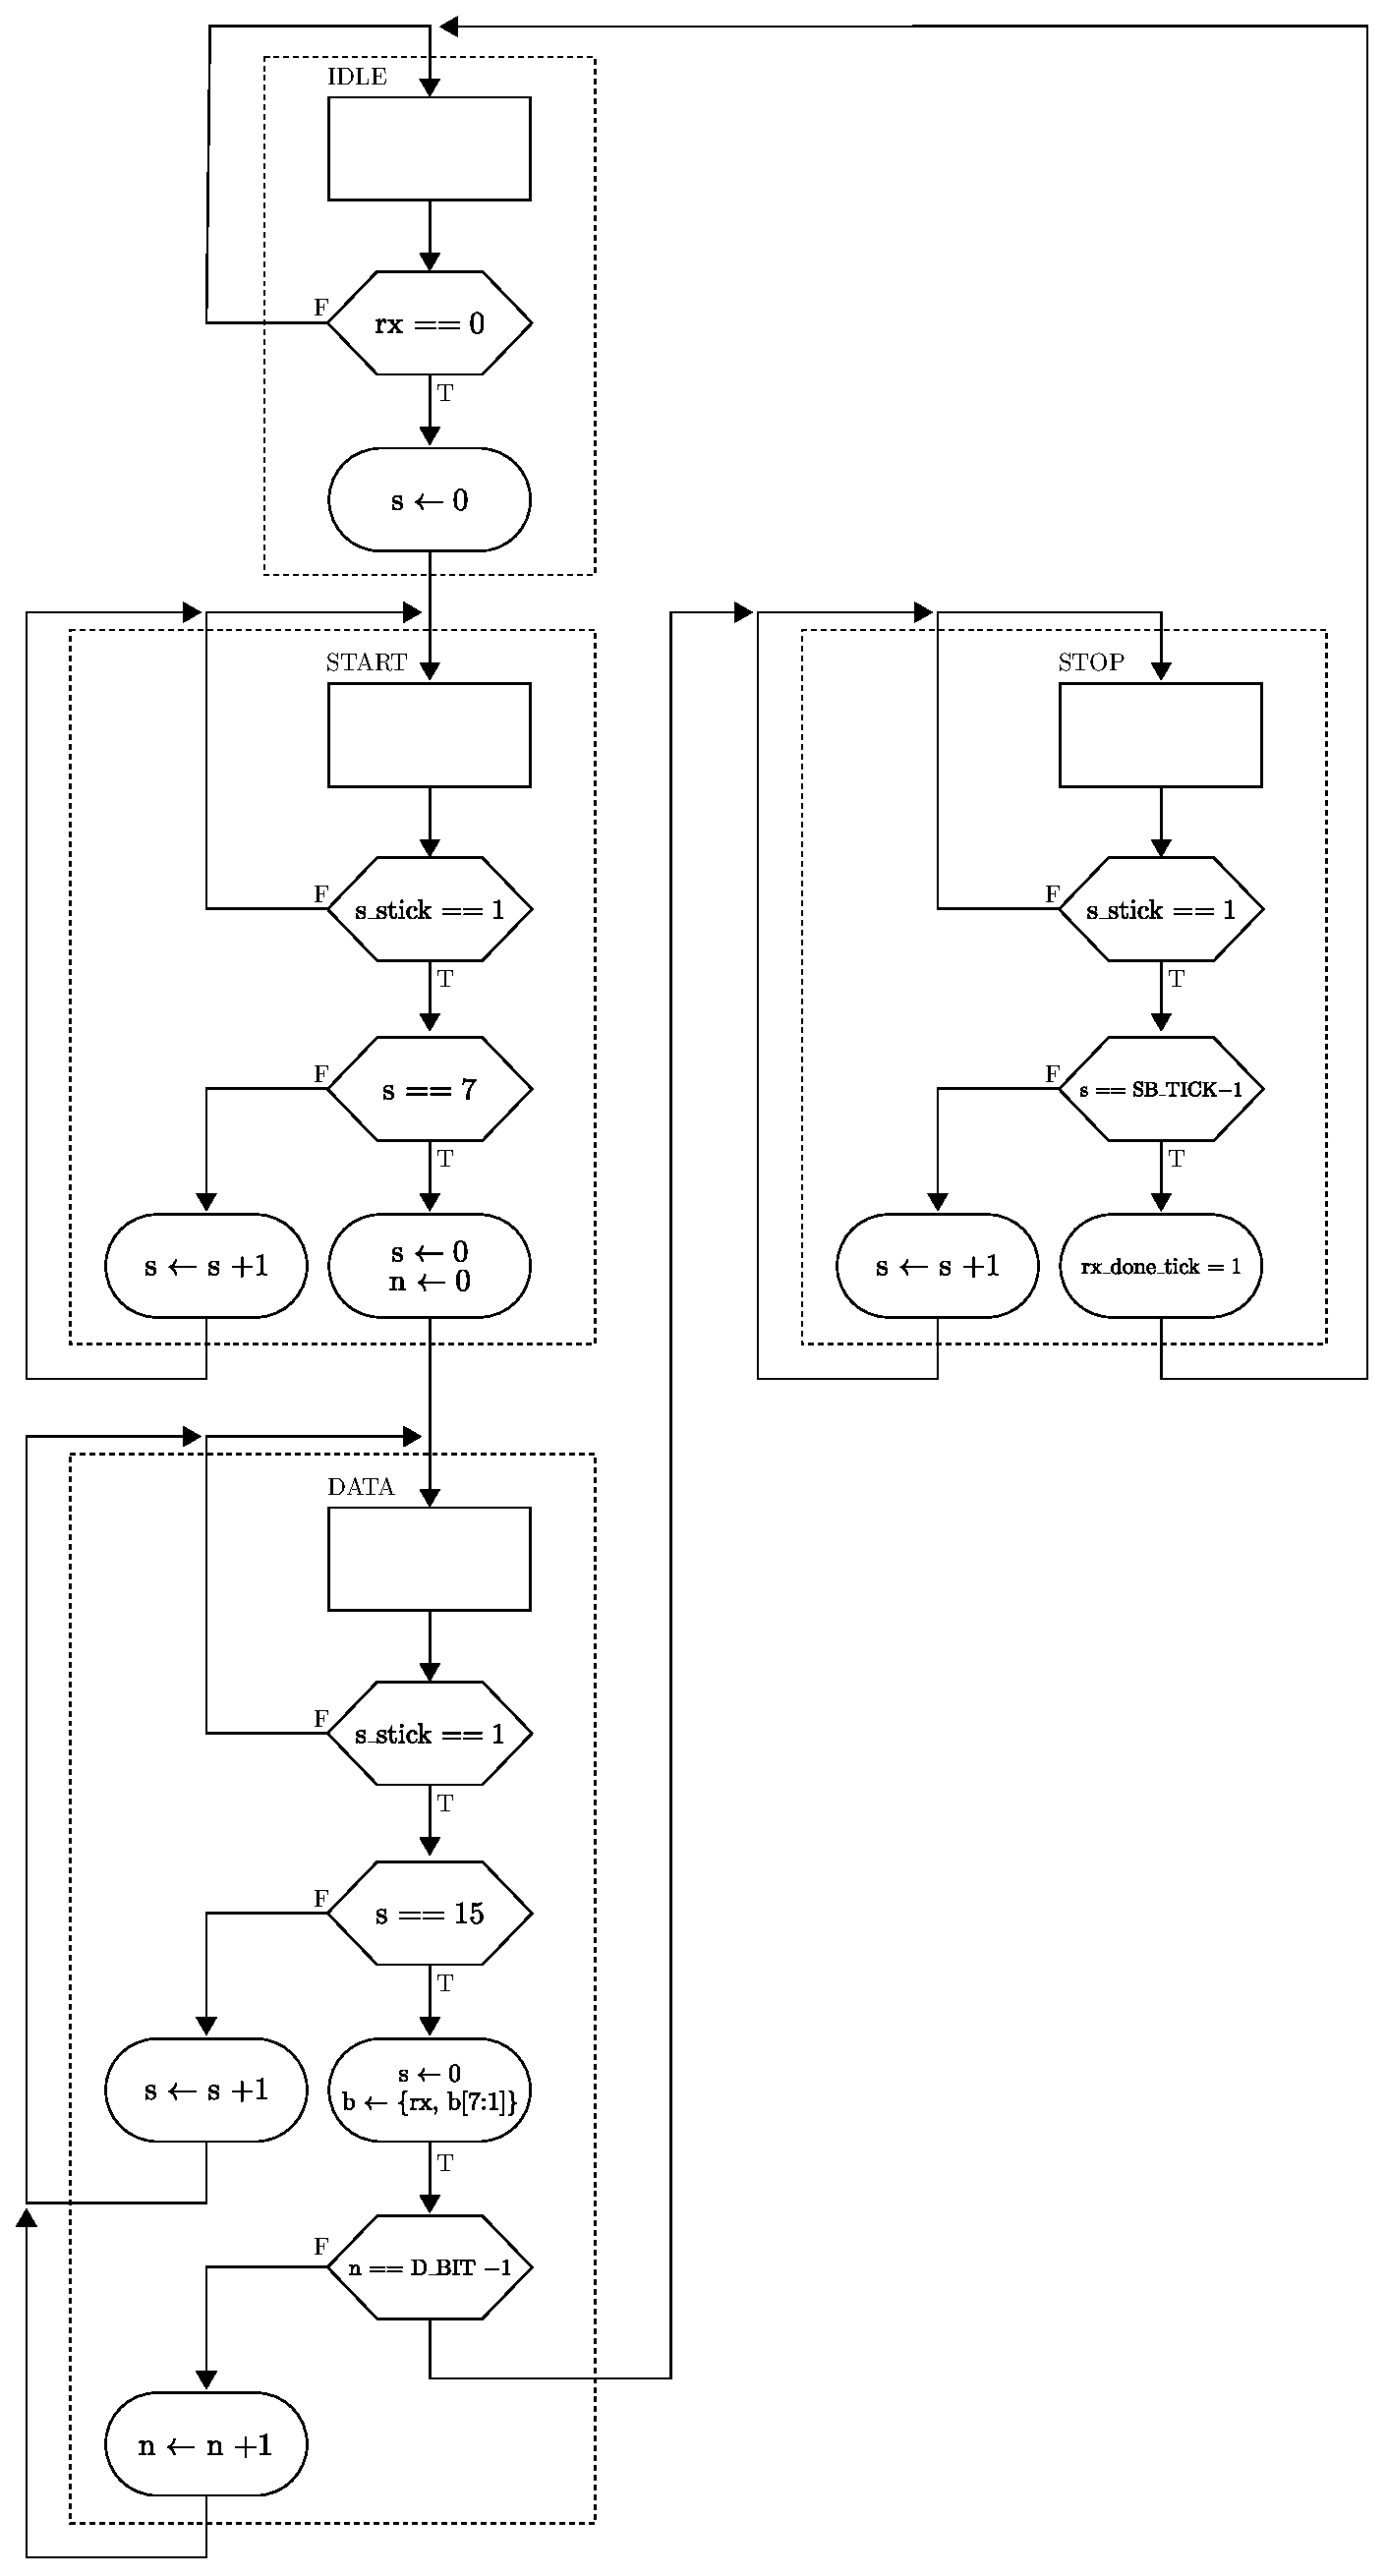
\includegraphics[width=0.75\textwidth]{asmd_uart_rx}
      \caption{Diagrama ASMD de receptor UART.}
      \label{fig:asmd_uart_rx}
    \end{figure}

    El diagrama sigue los pasos explicados en la Sección \ref{sec:sobremuestreo} e incluye tres estados principales: \textbf{START}, \textbf{DATA} y \textbf{STOP}, que representan el procesamiento del bit de inicio, los bits de datos y el bit de parada. La señal s\_tick es el tick de habilitación proveniente del generador de tasa de baudios, con 16 ticks en cada intervalo de bits. Es importante señalar que el FSMD permanece en el mismo estado a menos que se active la señal s\_tick. Existen dos contadores, representados por los registros s y n. El registro s lleva la cuenta de los ticks de muestreo, contando hasta 7 en el estado de START, hasta 15 en el estado de DATA, y hasta SB\_TICK en el estado de STOP. El registro n cuenta el número de bits de datos recibidos en el estado de DATA. Los bits recuperados se desplazan y se reensamblan en el registro b. Se incluye una señal de estado, rx\_done\_tick, que se activa durante un ciclo de reloj al finalizar el proceso de recepción. El código correspondiente se encuentra en el Código \ref{cod:uart_rx}.

    \subsection{Transmisor UART}
    
    La estructura de un subsistema de transmisión UART es similar a la del subsistema de recepción. Está compuesto por un transmisor UART y un generador de tasa de baudios.
    
    El transmisor UART es, en esencia, un registro de desplazamiento que envía los bits de datos a una velocidad específica. Esta velocidad puede ser controlada mediante ticks de habilitación de un solo ciclo de reloj generados por el generador de tasa de baudios. Como no se utiliza sobremuestreo, la frecuencia de los ticks es 16 veces más lenta que la del receptor UART. En lugar de introducir un nuevo contador, el transmisor UART suele compartir el generador de tasa de baudios del receptor y utiliza un contador interno para llevar el control de los ticks de habilitación. Se desplaza un bit cada 16 ticks de habilitación.
    
    El diagrama ASMD del transmisor UART es similar al del receptor UART. Tras la activación de la señal tx\_start, el FSMD carga la palabra de datos y avanza progresivamente por los estados de \textbf{START}, \textbf{DATA} y \textbf{STOP} para enviar los bits correspondientes. Al completar el proceso, se indica mediante la señal tx\_done\_tick, que se activa durante un ciclo de reloj. Se emplea un búfer de 1 bit, tx\_reg, para filtrar posibles fallos o errores. El código correspondiente se encuentra en el Código \ref{cod:uart_tx}.

	\section{Controlador SPI}

    El estándar SPI (Serial Peripheral Interface) o Interfaz Periférica Serial en español, es un protocolo de transferencia de datos en serie desarrollado originalmente por Motorola a principios de los 80. El bus SPI se compone de tres líneas, dos de ellas para transmitir y recibir datos en serie, y una para la señal de reloj. Se pueden conectar al bus un dispositivo maestro y varios dispositivos esclavos. El maestro genera la señal de reloj e inicia la transferencia de datos. El estándar SPI se utiliza ampliamente en sistemas embebidos para conectar módulos periféricos. \cite{Chu2018}, \cite{Chu2008}

    \subsection{Visión general}

    El estándar SPI especifica el protocolo que intercambia datos entre dos dispositivos a través de líneas seriales. En lugar de utilizar el esquema de sobremuestreo de UART, la interfaz SPI incluye una tercera línea para controlar el desplazamiento y el muestreo de los datos seriales. Las actividades se realizan en el flanco de transición de esta señal. Su función es similar a la señal de reloj de un sistema síncrono, por lo que esta línea se denomina reloj SPI.

    A diferencia de la configuración UART, en la que dos sistemas son simétricos y ambos pueden iniciar una transmisión, el estándar SPI utiliza una configuración maestro-esclavo. El maestro controla el funcionamiento general y genera la señal de reloj SPI. Sólo el maestro puede iniciar una transferencia de datos.

    A pesar de su nombre, el reloj SPI no es un reloj de sistema real y no debe utilizarse para controlar ningún registro directamente. La velocidad del reloj del sistema del controlador SPI es mucho más rápida que la velocidad del reloj SPI. Desde el punto de vista del controlador SPI, el reloj SPI es sólo otra señal de control.

    \subsection{Arquitectura del controlador}

    El diagrama conceptual de un bus SPI con dos dispositivos se muestra en la Figura \ref{fig:spi_diagram}. Tanto el maestro como el esclavo tienen un registro de desplazamiento (shift register) en su interior. Los dos registros de desplazamiento están conectados como un anillo a través de las líneas MOSI (para Master-Out-Slave-In) y MISO (para Master-In-Slave-Out) y su funcionamiento está coordinado por la misma señal de reloj SPI, SCLK. 

    Las señales MOSI y MISO son algo así como la señal de transmisión (TX) y la señal de recepción (RX) del UART. Suponemos que ambos registros tienen ocho bits de ancho y que la transferencia de datos se realiza byte a byte. Al principio de la operación, tanto el maestro como el esclavo cargan datos en los registros. Durante la transferencia de datos, los datos de ambos registros se desplazan un bit a la derecha en cada ciclo SCLK. Tras ocho ciclos SCLK, se han desplazado ocho bits de datos y el maestro y el esclavo han intercambiado los valores de los registros. A continuación, el maestro y el esclavo pueden procesar los datos recibidos. Esta operación puede interpretarse como que el maestro escribe datos en el esclavo y los lee simultáneamente, lo que se conoce como operación full-duplex.

    \begin{figure}[hbtp]
        \centering
        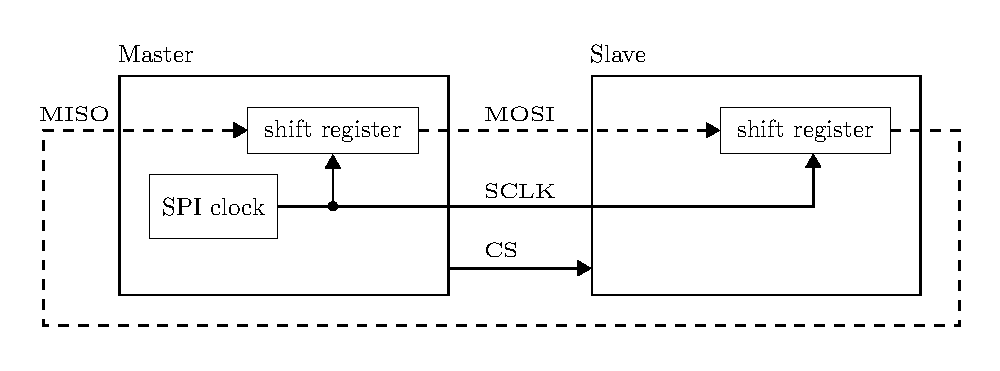
\includegraphics[width=0.8\textwidth]{spi_diagram}
        \caption{Diagrama conceptual del bus SPI.}
        \label{fig:spi_diagram}
    \end{figure}    

    Además de las líneas MOSI, MISO y SCLK, un dispositivo esclavo también puede tener una entrada de selección de chip activa en bajo, SS (para Slave Select). En otros casos también puede tener el nombre de  CS (para Chip-Select). Se puede utilizar para que el maestro seleccione el dispositivo esclavo deseado si hay varios dispositivos esclavos en el bus. Muchos dispositivos SPI también utilizan CS para ciertas funcionalidades de control y no se puede omitir, incluso en una configuración de un solo esclavo.

    \subsection{Configuración de múltiples dispositivos}

    El estándar SPI admite una configuración múltiple-esclavo, en la que un dispositivo maestro puede controlar más de un dispositivo esclavo. Existen dos esquemas básicos, que son la configuración en paralelo y la configuración en cadena.

    La configuración en paralelo utiliza una línea CS dedicada para cada dispositivo esclavo, como se muestra en la Figura \ref{fig:spi_parallel}. Una línea CS funciona como señal de selección de chip y el maestro puede seleccionar el dispositivo deseado activando la línea correspondiente. Esta configuración puede acomodar un maestro y dispositivos esclavos independientes. Dado que las líneas MISO de los esclavos están unidas, la línea MISO debe ser controlada por un buffer de tres estados y su salida debe estar en un estado de alta impedancia cuando el dispositivo esclavo no está seleccionado. 

    \begin{figure}[hbtp]
      \centering
      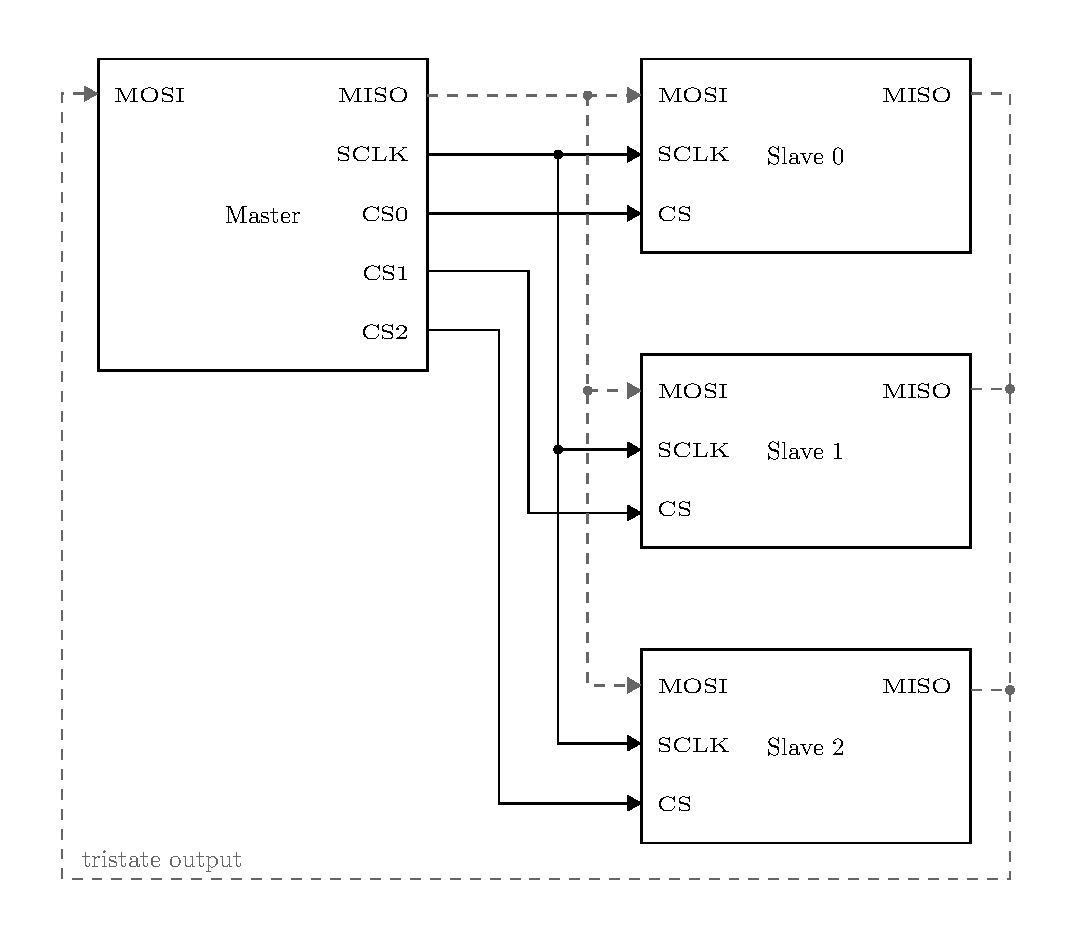
\includegraphics[width=0.8\textwidth]{spi_parallel}
      \caption{Configuración en paralelo de bus SPI.}
      \label{fig:spi_parallel}
    \end{figure}    

    La configuración en cadena conecta las líneas MOSI y MISO en una cadena en cascada, como se muestra en la Figura \ref{fig:spi_chain}. Se utiliza una única línea CS para controlar todos los dispositivos esclavos. Conceptualmente, la cadena forma un gran registro de desplazamiento y los datos se transfieren en serie de dispositivo a dispositivo. Los dispositivos de esta configuración deben ser cooperativos y seguir el mismo protocolo para transmitir, insertar y extraer bytes de datos.

    \begin{figure}[hbtp]
      \centering
      \includegraphics[width=0.8\textwidth]{spi_chain}
      \caption{Configuración en cadena de bus SPI.}
      \label{fig:spi_chain}
    \end{figure}    


    \subsection{Sincronización del controlador}

    El bus SPI utiliza los flancos del reloj SPI (SCLK) para controlar y sincronizar la transferencia de bits de los datos. Para aclarar la explicación, se definen dos actividades durante una transferencia de bits: enviar (es decir, desplazar) un nuevo bit a la línea de datos y muestrear (es decir, capturar) un bit de la línea de datos. El envío y el muestreo se completan en el mismo ciclo de reloj SPI, pero ocurren en flancos de reloj opuestos.
    En la Figura \ref{fig:spi_timing_diagram} se muestra un diagrama de tiempos representativo. Inicialmente, el bus está inactivo y la línea SCLK está en 0. En $t_{0}$, el maestro activa CS y el esclavo designado coloca el primer bit de datos (bit 7) en la línea MISO. En $t_{1}$, el maestro inicia el reloj SPI y envía el bit b7 en la línea MOSI.
Dado que la primera mitad del periodo del reloj SPI es 0, el valor en SCLK permanece sin cambios. El tiempo que transcurre entre $t_{0}$ y $t_{1}$ puede ser muy pequeño o incluso cero. En $t_{2}$, el maestro sube el reloj SPI y avanza a la segunda mitad del periodo del reloj. En el flanco de transición de 0 a 1, el maestro muestrea los datos en MISO y el esclavo los datos en MOSI. 
     En $t_{3}$, se completa el primer ciclo de reloj SPI. El maestro comienza el segundo periodo de reloj SPI y baja SCLK. Tanto el maestro como el esclavo envían nuevos bits a la línea de datos. En $t_{4}$, el maestro vuelve a subir SCLK y tanto el maestro como el esclavo muestrean los nuevos bits de datos. Las actividades de transmisión y muestreo se repiten hasta que se transfieren ocho bits de datos. Los últimos datos se muestrean en $t_{5}$ y SCLK vuelve a 0 en $t_{6}$. En $t_{7}$, el maestro desactiva CS. Cabe destacar que todos los muestreos se realizan en los flancos ascendentes de SCLK y todas las transmisiones (excepto la inicial) se realizan en los flancos descendentes de SCLK.

    \begin{figure}[hbtp]
      \centering
      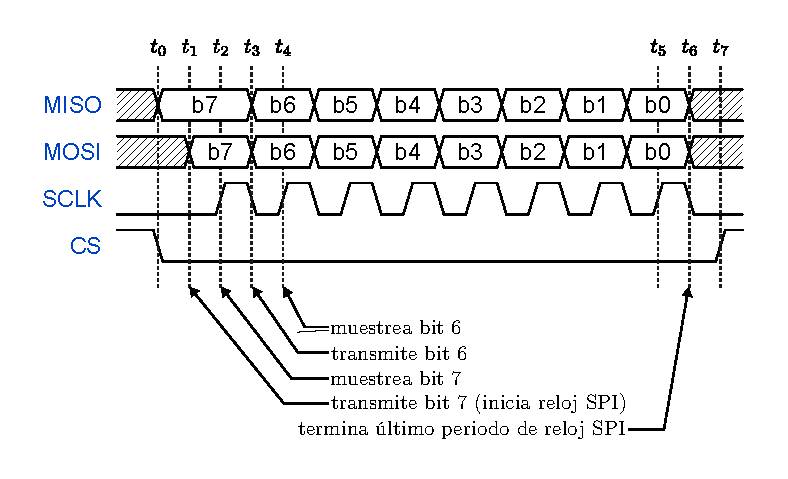
\includegraphics[width=0.8\textwidth]{spi_timing_diagram}
      \caption{Diagrama de tiempos representativo de una transferencia de datos SPI.}
      \label{fig:spi_timing_diagram}
    \end{figure}

    \subsection{Modos de operación}

    El modo de operación del SPI define las relaciones entre los flancos del reloj SPI y las actividades de envío y muestreo en las líneas de datos. Hay cuatro modos. Los modos dependen de dos parámetros, que son la polaridad del reloj (abreviado como CPOL, Clock Polarity) y la fase del reloj (abreviado como CPHA, Clock Phase). La polaridad del reloj se define como el valor de SCLK cuando está en reposo, que puede ser 0 o 1. La fase del reloj es más difícil de definir. Una interpretación es si un flanco del reloj se utiliza para enviar el primer bit de datos. Si CPHA es 1, el maestro conduce el bit en el primer flanco de transición. Si CPHA es 0, el maestro envía el bit en el flanco de transición cero, inmediatamente cuando CS se activa (lo que significa que no hay flanco o no en el primer flanco).

    Basándose en los dos parámetros, los modos de operación del SPI se definen como sigue:

    \begin{table}[h!]
      \caption{Modos de operación del SPI.}
      \begin{center}
      \resizebox{\textwidth}{!}{
        \begin{NiceTabular}{|c|c|c|c|c|}
          \hline
          \textbf{Modos SPI} & \textbf{Clock polarity} & \textbf{Clock phase } & \textbf{Los datos de desplazan en } & \textbf{Los datos se muestrean en }\\
                             & \textbf{(CPOL)}         & \textbf{(CPHA)}       &                                     & \\
          \hline
          0 & 0 & 0 & bajada SCLK, y cuando CS se activa & subida SCLK \\
          1 & 0 & 1 & subida SCLK & bajada SCLK \\
          2 & 1 & 0 & subida SCLK, y cuando CS se activa & bajada SCLK \\
          3 & 1 & 1 & bajada SCLK & subida SCLK \\
          \hline
        \end{NiceTabular}
      }
      \label{tab:spi_modes}
      \end{center}
    \end{table}

    Observe que el diagrama de tiempos de la Figura \ref{fig:spi_timing_diagram} corresponde al modo 0, ya que SCLK es 0 cuando está inactivo y el primer bit no es transmitido por el primer flanco de transición.

    El diagrama de tiempo de los cuatro modos se muestra en la Figura \ref{fig:spi_timing_diagram_modes}. El modo 0 es el modo más comúnmente utilizado. En este modo, el valor en reposo es 0 y el ciclo del reloj comienza con 0. Dado que el valor en reposo y el valor inicial del reloj son los mismos, el primer bit de datos se transmite antes del primer flanco de transición. En el modo 1, el valor en reposo también es 0, pero el ciclo del reloj comienza con 1. El valor inicial de 1 lleva a una transición de 0 a 1, por lo tanto, el primer bit se transmite en el primer flanco. Es importante notar que en estos dos modos, el período del reloj y el tiempo de inicio son los mismos, pero sus valores están fuera de fase.

    \begin{figure}[!h]
      \centering
      \includegraphics[width=0.85\textwidth]{spi_timing_diagram_modes}
      \caption{Diagrama de tiempos de los diferentes modos SPI.}
      \label{fig:spi_timing_diagram_modes}
    \end{figure}

    El valor en reposo de SCLK en los modos 2 y 3 es 1. La forma de onda de SCLK en el modo 2 es exactamente opuesta a la del modo 0, y la forma de onda en el modo 3 es exactamente opuesta a la del modo 1. Nuevamente, es importante destacar que el período del reloj y el tiempo de inicio son los mismos para todos los modos.

    \subsection{Aspectos indefinidos}

    La interfaz SPI fue desarrollada por Motorola y se ha convertido en un estándar de facto. No existe un organismo rector u organización que supervise este estándar. Varios aspectos importantes no están definidos en el estándar.

    El primer aspecto es el uso de la señal CS. La señal CS actúa principalmente como una señal de habilitación o selección de chip. Un dispositivo esclavo se desactiva si su señal CS no está activa. En muchos dispositivos, la señal CS también funciona como una señal de control. El intercambio de datos se realiza transacción por transacción:

    \begin{itemize}
      \item El maestro activa CS.
      \item El maestro y el esclavo seleccionado transfieren bits de datos.
      \item El maestro desactiva CS.
    \end{itemize}

    Una transacción se muestra en la Figura \ref{fig:spi_timing_diagram_aspects}. Las transiciones causadas por la activación y desactivación de CS se utilizan para activar ciertas acciones, como enviar un bit o capturar datos en paralelo, en el dispositivo esclavo. Esto implica que CS debe estar conectado al maestro, incluso si solo hay un dispositivo esclavo; es decir, simplemente conectarlo a 0 no funcionará. El estándar SPI no define explícitamente el papel de la señal CS ni el protocolo en la transacción. Además, los requisitos de temporización como el tiempo de preparación de CS ($\text{t}_{\text{SS\_SETUP}}$), que es el intervalo entre la activación de CS y el inicio del reloj, el tiempo de retención de CS ($\text{t}_{\text{SS\_HOLD}}$), que es el intervalo entre la desactivación de CS y la terminación del reloj, y el tiempo de cambio entre dos transacciones ($\text{t}_{\text{SS\_TURN}}$) no esta especificado.

    \begin{figure}[!h]
      \centering
      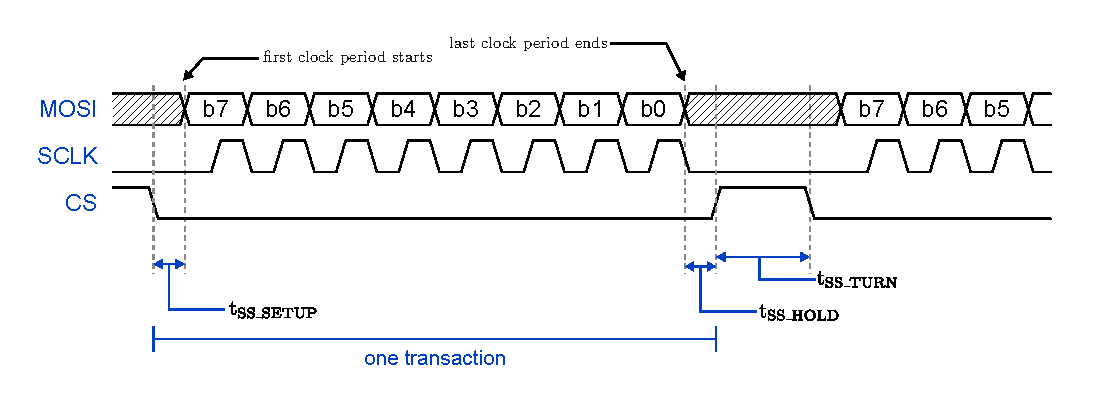
\includegraphics[width=0.95\textwidth]{spi_timing_diagram_aspects}
      \caption{Diagrama de tiempos con aspectos indefinidos, SPI modo 0.}
      \label{fig:spi_timing_diagram_aspects}
    \end{figure}

    El segundo aspecto indefinido es el número de bits en un intercambio de datos. En la Figura \ref{fig:spi_timing_diagram} se transfieren ocho bits. Sin embargo, el estándar SPI no especifica el número de bits transferidos en una transacción.

    Finalmente, el estándar SPI no especifica el orden de bits de la transmisión, es decir, si se transfiere primero el bit mas significactivo (MSB) o el bit menos significativo (LSB) de un byte de datos o de una palabra de datos. El MSB se utiliza comúnmente, pero no está garantizado.

    Debido a estos aspectos indefinidos, debemos consultar la hoja de datos del dispositivo y adaptar el acceso para cada dispositivo. Esto suele hacerlo el controlador de software y el programa de aplicación.


  \section{Convertidores DAC y ADC}

    \subsection{Visión general}

    Los convertidores analógico-digitales (ADC) traducen las magnitudes analógicas, características de la mayoría de los fenómenos del mundo real, a lenguaje digital, utilizado en el procesamiento de la información, la informática, la transmisión de datos y los sistemas de control. Los convertidores de digital-analógico (DAC) se utilizan para transformar los datos transmitidos o almacenados, o los resultados del procesamiento digital, de nuevo en variables del mundo real para su control, visualización de información o procesamiento analógico posterior \cite{Kester2007}.

    Las variables de entrada analógicas, independientemente de su su origen, suelen ser convertidas mediante transductores en voltajes o corrientes. Estas magnitudes eléctricas pueden manifestarse de las siguientes formas: (1) como mediciones directas y continuas de corriente continua (DC) que pueden ser rápidas o lentas, representando un fenómeno en el dominio del tiempo, (2) como formas de onda de corriente alterna (AC) moduladas mediante diversas técnicas de modulación, (3) o en una combinación de ambas. Ejemplos del primer tipo incluyen las salidas de termopares, potenciómetros en referencias de corriente continua (DC); del segundo tipo, mediciones ópticas moduladas, puentes de corriente alterna (AC), y señales digitales sumergidas en ruido.

    Las variables analógicas a tratar son aquellas que involucran voltajes o corrientes que representan fenómenos analógicos reales. Estas pueden ser de banda ancha o banda estrecha, y pueden ser escaladas a partir de la medición directa o sometidas a algún tipo de preprocesamiento analógico, como la linealización, combinación, demodulación, filtrado, retención de muestras, entre otros.

    Como parte del proceso, los voltajes y corrientes se normalizan a rangos compatibles con los rangos de entrada asignados al ADC. Las salidas analógicas de voltaje o corriente de los DACs se generan de forma directa y en formato normalizado, aunque pueden ser procesadas posteriormente (por ejemplo, escaladas, filtradas, amplificadas, etc.)

    La información en forma digital se representa normalmente mediante niveles de voltaje arbitrariamente fijos referidos a tierra, ya sea en las salidas de las compuertas lógicas o aplicados a sus entradas. Los números digitales utilizados son básicamente binarios; es decir, cada bit o unidad de información tiene uno de dos posibles estados. Estos estados son apagado, falso, o 0, y encendido, verdadero, o 1. También es posible representar los dos estados lógicos mediante dos niveles diferentes de corriente; sin embargo, esto es mucho menos común que el uso de voltajes. Tampoco es necesario que los voltajes estén referidos a tierra, como en el caso de la lógica acoplada por emisor (ECL), la lógica acoplada por emisor positiva (PECL) o la lógica de señalización diferencial de bajo voltaje (LVDS).

    \subsection{Códificación}

    Una palabra o \textit{Word} en inglés, es grupo de niveles que representan un número digital. Estos niveles pueden presentarse de forma simultánea en \textit{paralelo}, en un bus o en grupos de entradas o salidas de compuertas, de forma \textit{serial} (es decir, en una secuencia temporal) en una única línea, o como una secuencia de bytes paralelos (serial por bytes) o nibbles (porciones más pequeñas de bytes). Por ejemplo, una palabra de 16 bits puede ocupar los 16 bits de un bus de 16 bits, dividirse en dos bytes secuenciales para un bus de 8 bits, o en cuatro nibbles de 4 bits para un bus de 4 bits.

    A cada nivel analógico cuantificado (es decir, que representa una porción única del rango analógico) se le asigna una agrupación, ya sea paralelo o en serie única de niveles digitales, o un \textit{número} o \textit{código}. Un código digital típico sería el siguiente arreglo:

    \begin{equation}
      a_{7} \; a_{6} \; a_{4} \; a_{3} \; a_{2} \; a_{1} \; a_{0} = 1 \; 0 \; 1 \; 1 \; 1 \; 0 \; 0 \; 1
    \end{equation}

    Está compuesto por ocho bits. El ``1'' en el extremo izquierdo se denomina ``bit más significativo'' (MSB, o Bit 1), mientras que el del extremo derecho se llama ``bit menos significativo'' (LSB, o Bit N: 8 en este caso). El significado del código, ya sea como un número, un carácter o una representación de una variable analógica, no se conoce hasta que se defina tanto el \textit{código} como su \textit{relación de conversión}. Es importante no confundir la designación de un bit específico (como Bit 1, Bit 2, etc.) con los subíndices asociados al arreglo ``a''. Estos subíndices corresponden a la potencia de 2 vinculada al peso de cada bit dentro de la secuencia.

    El código más conocido, aparte del sistema decimal (base 10), es el binario natural o directo (base 2). Los códigos binarios son más utilizados para representar números enteros. En un código binario natural de N bits, el LSB tiene un peso de $2^{0}$ (es decir, 1), el siguiente bit tiene un peso de $2^{1}$ (o 2), y así sucesivamente hasta llegar al MSB, cuyo peso es de $2^{N-1}$ (o $2^{N} / 2$). El valor de un número binario se obtiene sumando los pesos de todos los bits no nulos. Cuando estos bits ponderados se suman, forman un número único que puede variar entre 0 y $2^{N} -1$. Cada bit adicional en cero al final, si existe, esencialmente duplica el tamaño del número.

    En la tecnología de convertidores, el valor de escala completa (abreviado como FS) es independiente del número de bits de resolución, N. Un sistema de codificación más práctico es el binario fraccionario, que siempre se normaliza a la escala completa. El binario entero puede interpretarse como binario fraccionario dividiendo todos los valores enteros por $2^{N}$. Por ejemplo, el MSB tiene un peso de $1/2$ (es decir, $2^{(N-1)}/2^{N}= 2^{-1}$), el siguiente bit tiene un peso de $1/4$ (o $2^{-2}$), y así sucesivamente hasta el LSB, que tiene un peso de $1/2^{N}$ (o $2^{-N}$). Al sumar los bits ponderados, se obtiene un número con cualquiera de los $2^{N}$ valores, que van desde 0 hasta ($1 - 2^{-N}$) de la escala completa. Los bits adicionales simplemente añaden mayor detalle sin modificar el rango de la escala completa. La relación entre los números en base 10 y los números binarios (base 2) se ilustra en las siguientes ecuaciones:

    \begin{equation}
      \text{Numbero entero}_{\;10} = \underbrace{a_{N-1} 2^{N-1}}_{\text{MSB}}  + a_{N-2} 2^{N-2} + \ldots + a_{1} 2^{1} + \underbrace{a_{0} 2^{0}}_{\text{LSB}} 
    \end{equation}

    \begin{equation}
      \text{Numbero fraccionario}_{\;10} = \underbrace{a_{N-1} 2^{-1}}_{\text{MSB}}  + a_{N-2} 2^{-2} + \ldots + a_{1} 2^{-(N-1)} + \underbrace{a_{0} 2^{-N}}_{\text{LSB}} 
    \end{equation}

  
    En los sistemas de conversión de datos, el método de codificación debe estar relacionado con el rango de entrada analógica (o intervalo) de un ADC, o con el rango de salida analógica de un DAC. El caso más sencillo ocurre cuando la entrada del ADC o la salida del DAC es una tensión unipolar positiva (aunque las salidas de corriente son comunes en los DACs, no lo son tanto en las entradas de ADCs). El código más utilizado para este tipo de señal es el binario directo, como se muestra en la Tabla \ref{tab:adc_codigos_unipolares} para un convertidor de 4 bits. Como se puede observar, existen 16 niveles distintos posibles, desde el código 0000 (todos ceros) hasta el código 1111 (todos unos). Es importante destacar que el valor analógico representado por el código de todos unos no corresponde a la escala completa (FS), sino a FS menos 1 LSB. Esta es una convención común en la notación de conversión de datos, aplicable tanto a ADCs como a DACs. La Tabla \ref{tab:adc_codigos_unipolares} muestra el número equivalente en base 10, el valor del código binario en base 2 en relación a la escala completa (FS), y el nivel de voltaje correspondiente para cada código (suponiendo un convertidor de escala completa de 10 V). También se muestra el código Gray equivalente, que será discutido más adelante

    \begin{table}[h!]
      \caption{Códigos binarios unipolares, convertidor de 4 bits.}
      \begin{center}
      \resizebox{\textwidth}{!}{
        \begin{NiceTabular}{|c|c|c|c|c|}
        \hline
          \textbf{Número en base 10} & \textbf{Escala} & \textbf{+10V FS} & \textbf{Binario} & \textbf{Gray} \\ 
        \hline
        +15 & +FS – 1LSB = +15/16 FS & 9.375 & 1111 & 1000 \\ 
        +14 & +7/8 FS & 8.750 & 1110 & 1001 \\ 
        +13 & +13/16 FS & 8.125 & 1101 & 1011 \\ 
        +12 & +3/4 FS & 7.500 & 1100 & 1010 \\ 
        +11 & +11/16 FS & 6.875 & 1011 & 1110 \\ 
        +10 & +5/8 FS & 6.250 & 1010 & 1111 \\ 
        +9 & +9/16 FS & 5.625 & 1001 & 1101 \\ 
        +8 & +1/2 FS & 5.000 & 1000 & 1100 \\ 
        +7 & +7/16 FS & 4.375 & 0111 & 0100 \\ 
        +6 & +3/8 FS & 3.750 & 0110 & 0101 \\ 
        +5 & +5/16 FS & 3.125 & 0101 & 0111 \\ 
        +4 & +1/4 FS & 2.500 & 0100 & 0110 \\ 
        +3 & +3/16 FS & 1.875 & 0011 & 0010 \\ 
        +2 & +1/8 FS & 1.250 & 0010 & 0011 \\ 
        +1 & 1LSB = +1/16 FS & 0.625 & 0001 & 0001 \\ 
        0 & 0 & 0.000 & 0000 & 0000 \\ 
        \hline
        \end{NiceTabular}
      }
      \label{tab:adc_codigos_unipolares}
      \end{center}
    \end{table}

    \subsection{Cuantización}

    La Figura \ref{fig:adc_dac_3bits} muestra la función de transferencia de un DAC ideal de 3 bits con codificación binaria directa en la entrada. Se puede observar que la salida analógica es cero cuando el código de entrada es todo ceros. A medida que el código de entrada digital aumenta, la salida analógica incrementa 1 LSB (equivalente a 1/8 de la escala en este caso) por cada cambio de código. El voltaje de salida más alto es de 7/8 de la escala completa (FS), lo que corresponde a un valor de FS - 1 LSB. La salida a mitad de escala, equivalente a 1/2 FS, se produce cuando el código de entrada digital es 100.

    \begin{figure}[!h]
      \centering
      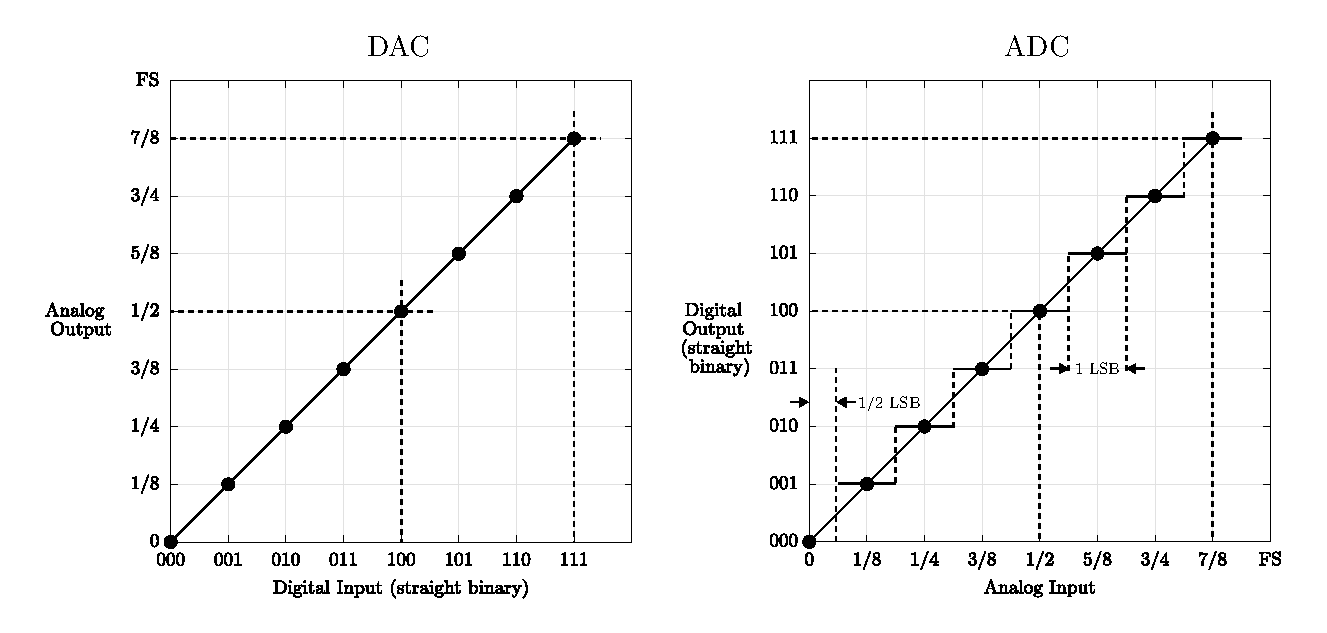
\includegraphics[width=0.95\textwidth]{adc_dac_3bits}
      \caption{Funciones de transferencia para un DAC y ADC unipolares de 3 bits.}
      \label{fig:adc_dac_3bits}
    \end{figure}

    La función de transferencia de un ADC ideal de 3 bits se ilustra en la Figura \ref{fig:adc_dac_3bits}. En este caso, existe un rango de voltaje de entrada analógico dentro del cual el ADC genera un código de salida específico; este rango, conocido como \textit{incertidumbre de cuantización}, es equivalente a 1 LSB. Es importante destacar que, en un ADC ideal, la amplitud de las regiones de transición entre códigos adyacentes es cero. No obstante, en la práctica, siempre hay ruido de transición asociado a estos niveles, lo que provoca que la amplitud no sea nula. Por convención, la entrada analógica correspondiente a un código determinado se define por el \textit{centro del código}, ubicado a medio camino entre dos regiones de transición adyacentes (representado por los puntos negros en el diagrama). Esto implica que la primera región de transición se produce a $1/2$ LSB. El voltaje de entrada analógico de escala completa se establece en 7/8 FS (FS - 1 LSB).

    Otro código que merece ser mencionado es el código Gray (o binario reflejado). El equivalente del código binario directo de 4 bits en código Gray también se ilustra en la Tabla \ref{tab:adc_codigos_unipolares}. Aunque su uso en aritmética de computadoras es poco común, el código Gray posee propiedades que lo hacen útil en la conversión A/D. Una característica destacada es que, en el código Gray, cuando el valor del número cambia, las transiciones de un código al siguiente afectan solo a un bit a la vez. Esto es en contraste con el código binario, donde todos los bits cambian en la transición entre 0111 y 1000. Algunos ADCs lo emplean de manera interna y luego lo convierten a código binario para su uso externo.

    \subsection{Códigos binarios}

    En muchos sistemas, es deseable representar cantidades analógicas tanto positivas como negativas mediante códigos binarios. Existen varios métodos para lograr esto, como el binario con desplazamiento, el complemento a dos, el complemento a uno o la magnitud con signo, aunque los más comunes son el binario con desplazamiento y el complemento a dos. Las relaciones entre estos códigos para un sistema de 4 bits se ilustran en la Tabla \ref{tab:codigos_bipolares}. Es importante destacar que los valores están ajustados para un rango de voltaje de entrada/salida de $\pm 5$ V en escala completa.

    \begin{table}[h!]
      \caption{Códigos bipolares, convertidor de 4 bits.}
      \begin{center}
      \resizebox{\textwidth}{!}{
        \begin{NiceTabular}{|c|c|c|c|c|c|c|}
        \hline
          \textbf{Número en base 10} & \textbf{Escala} & \textbf{$\pm$5V FS} & \textbf{Offset binary} & \textbf{Twos comp} & \textbf{Ones comp} & \textbf{Sign Mag} \\ 
        \hline
        +7 & +FS - 1LSB = +7/8 FS & +4.375 & 1111 & 0111 & 0111 & 0111 \\ 
        +6 & +3/4 FS & +3.750 & 1110 & 0110 & 0110 & 0110 \\ 
        +5 & +5/8 FS & +3.125 & 1101 & 0101 & 0101 & 0101 \\ 
        +4 & +1/2 FS & +2.500 & 1100 & 0100 & 0100 & 0100 \\ 
        +3 & +3/8 FS & +1.875 & 1011 & 0011 & 0011 & 0011 \\ 
        +2 & +1/4 FS & +1.250 & 1010 & 0010 & 0010 & 0010 \\ 
        +1 & +1/8 FS & +0.625 & 1001 & 0001 & 0001 & 0001 \\ 
        0 & 0 & 0.000 & 1000 & 0000 & *0000 & *1000 \\ 
        -1 & -1/8 FS & -0.625 & 0111 & 1111 & 1110 & 1001 \\ 
        -2 & -1/4 FS & -1.250 & 0110 & 1110 & 1101 & 1010 \\ 
        -3 & -3/8 FS & -1.875 & 0101 & 1101 & 1100 & 1011 \\ 
        -4 & -1/2 FS & -2.500 & 0100 & 1100 & 1011 & 1100 \\ 
        -5 & -5/8 FS & -3.125 & 0011 & 1011 & 1010 & 1101 \\ 
        -6 & -3/4 FS & -3.750 & 0010 & 1010 & 1001 & 1110 \\ 
        -7 & -FS + 1LSB = -7/8 FS & -4.375 & 0001 & 1001 & 1000 & 1111 \\ 
        -8 & -FS & -5.000 & 0000 & 1000 &  &  \\ 
        \hline
        \end{NiceTabular}
      }
      \label{tab:codigos_bipolares}
      \end{center}
    \end{table}

    En el sistema binario con desplazamiento, el valor de señal cero se asigna al código 1000. La secuencia de códigos es idéntica a la del binario directo, siendo la única diferencia el desplazamiento de media escala asociado a la señal analógica. El valor más negativo (–FS + 1 LSB) se representa con el código 0001, mientras que el valor más positivo (+FS – 1 LSB) se representa con el código 1111. Es importante señalar que, para mantener una simetría perfecta alrededor de la mitad de la escala, el código de todos ceros (0000), que representa la escala completa negativa (–FS), generalmente no se utiliza en los cálculos. Puede emplearse para indicar una condición de fuera de rango negativa o asignarse simplemente el valor de 0001 (–FS + 1 LSB).


    La relación entre el código binario con desplazamiento y el rango de salida analógica de un DAC bipolar de 3 bits se muestra en la Figura \ref{fig:adc_dac_3bits_offset}. La salida analógica del DAC es cero cuando el código de entrada es 100. El voltaje de salida más negativo suele estar definido por el código 001 (–FS + 1 LSB), mientras que el más positivo lo define el código 111 (+FS – 1 LSB). El voltaje de salida correspondiente al código de entrada 000 se puede utilizar si se desea, pero esto provoca que la salida no sea simétrica respecto al cero y complica los cálculos.

    El código de salida binario con desplazamiento para un ADC bipolar de 3 bits, en función de su entrada analógica, se muestra en la Figura \ref{fig:adc_dac_3bits_offset}. Es importante señalar que la entrada analógica cero define el centro del código de mitad de escala, que es 100. Al igual que en los DACs bipolares, el voltaje de entrada más negativo está definido por el código 001 (–FS + 1 LSB), mientras que el más positivo lo define el código 111 (+FS – 1 LSB). Como se mencionó anteriormente, el código de salida 000 está disponible para su uso si se desea, pero esto provoca que la salida no sea simétrica respecto al cero y complica los cálculos matemáticos

    \begin{figure}[!h]
      \centering
      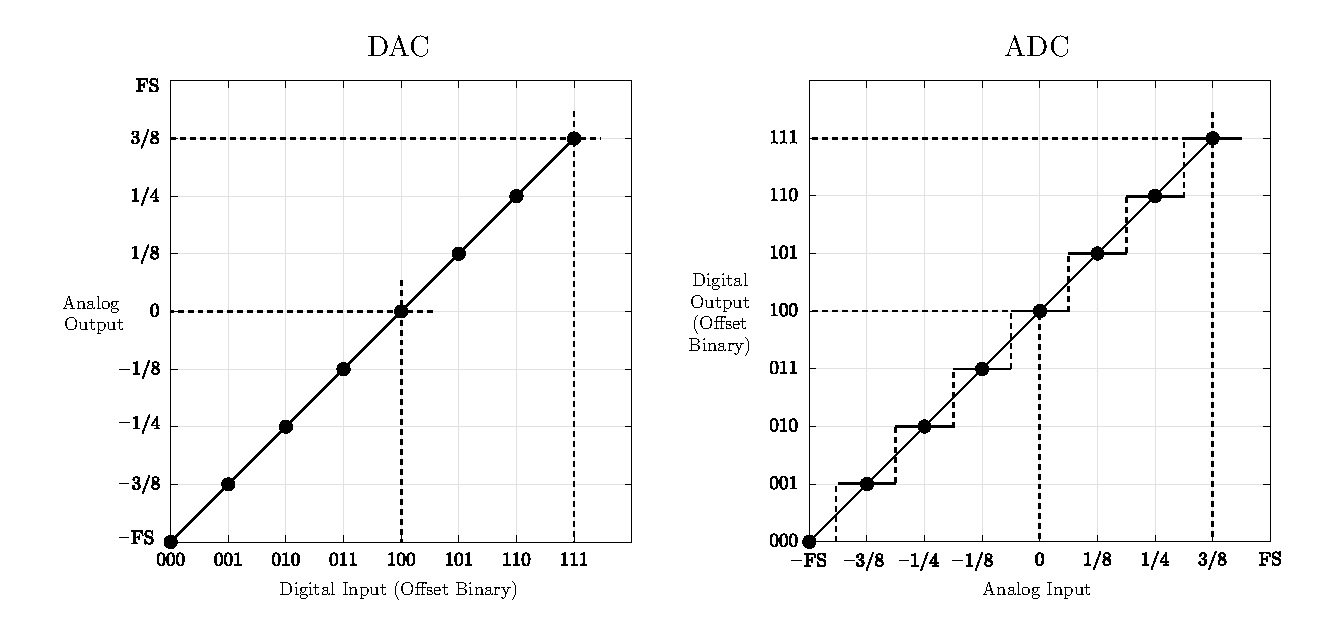
\includegraphics[width=0.95\textwidth]{adc_dac_3bits_offset}
      \caption{Funciones de transferencia para un DAC y ADC bipolares ideales de 3 bits.}
      \label{fig:adc_dac_3bits_offset}
    \end{figure}

    El complemento a dos es idéntico al binario con desplazamiento, con la diferencia de que el bit más significativo (MSB) se invierte. Esto es muy fácil de implementar en un conversor de datos mediante un inversor simple o utilizando la salida complementaria de un flip-flop tipo D. La popularidad del complemento a dos radica en la facilidad con la que se pueden realizar operaciones matemáticas en computadoras y procesadores DSP. En términos de conversión, el complemento a dos se compone de un código binario para magnitudes positivas (bit de signo 0) y el complemento a dos de cada número positivo para representar su equivalente negativo. El complemento a dos se forma aritméticamente invirtiendo el número y sumando 1 LSB. Por ejemplo, para obtener –3/8 de FS, se toma el complemento a dos de +3/8 de FS. Primero se invierte +3/8 de FS, es decir, 0011, obteniendo 1100. Luego, al sumar 1 LSB, obtenemos 1101. El complemento a dos simplifica las operaciones de resta. Por ejemplo, para restar 3/8 de FS de 4/8 de FS, se suma 4/8 a –3/8, es decir, se suman 0100 y 1101. El resultado es 0001, que equivale a 1/8, ignorando el acarreo adicional.

    El complemento a uno también puede emplearse para representar números negativos, aunque es mucho menos común que el complemento a dos y su uso es raro en la actualidad. El complemento a uno se obtiene simplemente invirtiendo todos los dígitos de un número positivo. Por ejemplo, el complemento a uno de 3/8 FS (0011) es 1100. Un código con complemento a uno se forma invirtiendo cada valor positivo para generar su valor negativo correspondiente. Esto incluye el cero, que puede representarse con dos códigos: 0000 (conocido como 0+) o 1111 (conocido como 0–). Esta ambigüedad debe resolverse matemáticamente, lo que presenta problemas obvios para los ADCs y DACs, donde solo existe un código para representar el valor cero.

    La representación de magnitud con signo podría parecer la forma más sencilla de expresar digitalmente cantidades analógicas con signo. Consiste simplemente en determinar el código adecuado para la magnitud y añadir un bit de polaridad. El sistema BCD de magnitud con signo es común en voltímetros digitales bipolares, pero presenta el problema de tener dos códigos posibles para representar el valor cero. Por este motivo, no es muy popular en la mayoría de las aplicaciones que involucran ADCs o DACs.

    \subsection{Resolución}

    Lo más importante a tener en cuenta sobre los DACs y ADCs es que, ya sea la entrada o la salida, es digital, lo que significa que la señal está cuantizada. En otras palabras, una palabra de N bits representa uno de los $2^N$ estados posibles. Por lo tanto, un DAC de N bits (con una referencia fija) solo puede generar $2^N$ salidas analógicas posibles, y un ADC de N bits solo puede producir $2^N$ salidas digitales. Como se mencionó anteriormente, las señales analógicas generalmente serán voltajes o corrientes.

    La resolución de los convertidores de datos puede expresarse de diversas maneras: en términos del peso del bit menos significativo (LSB), en partes por millón de la escala completa (ppm FS), en milivoltios (mV), entre otros. Dado que los dispositivos, incluso los provenientes del mismo fabricante, pueden tener especificaciones diferentes, los usuarios de convertidores deben aprender a interpretar y convertir entre estos distintos tipos de especificaciones para poder comparar dispositivos con éxito.

    Antes de analizar las distintas arquitecturas utilizadas en los convertidores de datos, es necesario evaluar el rendimiento que se puede esperar y las especificaciones que resultan importantes. En las siguientes secciones se abordará la definición de los errores y las especificaciones asociadas a los convertidores de datos. Comprender esto es fundamental para identificar las fortalezas y debilidades de las distintas arquitecturas de ADC/DAC.

    La Figura \ref{fig:funcion_de_transferencia} muestra las características de transferencia ideales de un DAC unipolar de 3 bits y un ADC unipolar de 3 bits. En un DAC, tanto la entrada como la salida están cuantizadas, por lo que el gráfico consta de ocho puntos. Si bien es posible discutir la línea que conecta estos puntos, es fundamental recordar que la característica de transferencia real no es una línea continua, sino un conjunto de puntos discretos.

    \begin{figure}[!h]
      \centering
      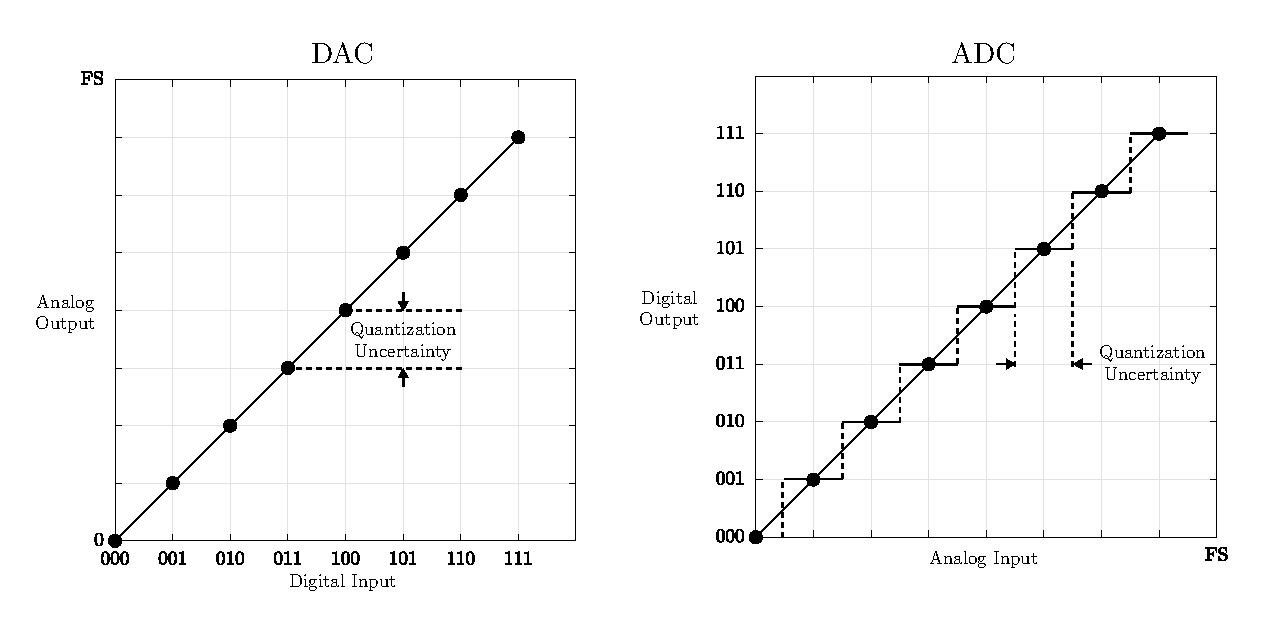
\includegraphics[width=0.95\textwidth]{funcion_de_transferencia}
      \caption{Funciones de transferencia para DAC y ADC ideales de 3 bits.}
      \label{fig:funcion_de_transferencia}
    \end{figure}

    La entrada de un ADC es analógica y no está cuantizada, mientras que su salida sí lo está. Por ello, la característica de transferencia se representa mediante ocho escalones horizontales. Para analizar el desplazamiento, la ganancia y la linealidad de un ADC, se considera la línea que une los puntos medios de estos escalones, conocidos habitualmente como los \textit{centros de código}.

    \subsection{Errores en los convertidores}

    En los DACs y ADCs, la escala completa digital (todos los bits en 1) corresponde a 1 LSB por debajo de la escala completa analógica (FS). Las transiciones ideales en un ADC ocurren a 1/2 LSB por encima de cero y, a partir de ahí, en cada LSB hasta llegar a $1 \frac{1}{2}$ LSB por debajo de la escala completa analógica. Como la entrada analógica de un ADC puede tomar cualquier valor, mientras que la salida digital está cuantizada, puede haber una diferencia de hasta 1/2 LSB entre la entrada analógica real y el valor exacto de la salida digital. Este fenómeno se conoce como \textit{error de cuantización} o \textit{incertidumbre de cuantización}, como se muestra en la Figura \ref{fig:funcion_de_transferencia}. En aplicaciones de señal alterna (muestreo), este error de cuantización genera ruido de cuantización.

    Los cuatro errores de corriente continua en un convertidor de datos son: \textit{error de offset}, \textit{error de ganancia} y dos tipos de \textit{errores de linealidad} (\textit{diferencial} e \textit{integral}). Los errores de offset y ganancia son similares a los que se presentan en amplificadores, para un rango de entrada bipolar. (Cabe señalar que, aunque los errores de offset y de cero son idénticos en amplificadores y convertidores de datos unipolares, no lo son en convertidores bipolares, por lo que deben diferenciarse con cuidado).

    Las características de transferencia tanto de los DACs como de los ADCs pueden representarse como una línea recta expresada por D = K + GA, donde D es el código digital, A es la señal analógica, y K y G son constantes. En un convertidor unipolar, el valor ideal de K es cero; en un convertidor bipolar con offset, es –1 LSB. El error de offset es la diferencia entre el valor real de K y su valor ideal.

    El error de ganancia es la diferencia entre G y su valor ideal, y generalmente se expresa como un porcentaje de esa diferencia, aunque también puede definirse como la contribución del error de ganancia (en mV o LSB) al error total en escala completa. Estos errores suelen poder corregirse por el usuario del convertidor de datos. Sin embargo, es importante señalar que en los amplificadores, el ajuste de desfase se realiza con una entrada de cero, mientras que la ganancia se ajusta cerca de la escala completa. El algoritmo de ajuste para un convertidor de datos bipolar es más complejo.

    El error de linealidad integral de un convertidor es similar al error de linealidad de un amplificador, y se define como la desviación máxima de la característica de transferencia real del convertidor respecto a una línea recta, generalmente expresada como un porcentaje de la escala completa (aunque también puede expresarse en LSBs). En el caso de un ADC, la convención más común es trazar una línea recta a través de los puntos medios de los códigos, o centros de código. Hay dos métodos comunes para determinar esta línea recta: la línea basada en los puntos extremos y la mejor línea recta.

    El otro tipo de no linealidad en un convertidor es la no linealidad diferencial (DNL), que se refiere a la linealidad de las transiciones de código en el convertidor. Idealmente, un cambio de 1 LSB en el código digital debería corresponder a un cambio exacto de 1 LSB en la señal analógica. En un DAC, esto significa que un cambio de 1 LSB en el código digital genera exactamente 1 LSB de cambio en la salida analógica, mientras que en un ADC se requiere un cambio de 1 LSB en la entrada analógica para pasar de una transición digital a la siguiente. El error de linealidad diferencial se define como la desviación máxima de cualquier cambio cuántico (o de LSB) en toda la función de transferencia con respecto a su tamaño ideal de 1 LSB.

    Cuando el cambio en la señal analógica correspondiente a un cambio de 1 LSB en el código digital es mayor o menor que 1 LSB, se considera que existe un error de DNL. El error de DNL en un convertidor se define generalmente como el valor máximo de DNL que puede encontrarse en cualquier transición dentro del rango del convertidor. La Figura \ref{fig:funcion_de_transferencia_no_ideal} muestra las funciones de transferencia no ideales de un DAC y un ADC, mostrando los efectos del error de DNL.

    Si el DNL de un DAC es inferior a –1 LSB en alguna transición, el DAC se considera no monótono, lo que significa que su característica de transferencia presenta uno o más máximos o mínimos localizados. Un DNL superior a +1 LSB no provoca no monotonía, pero sigue siendo indeseable

    \begin{figure}[!h]
      \centering
      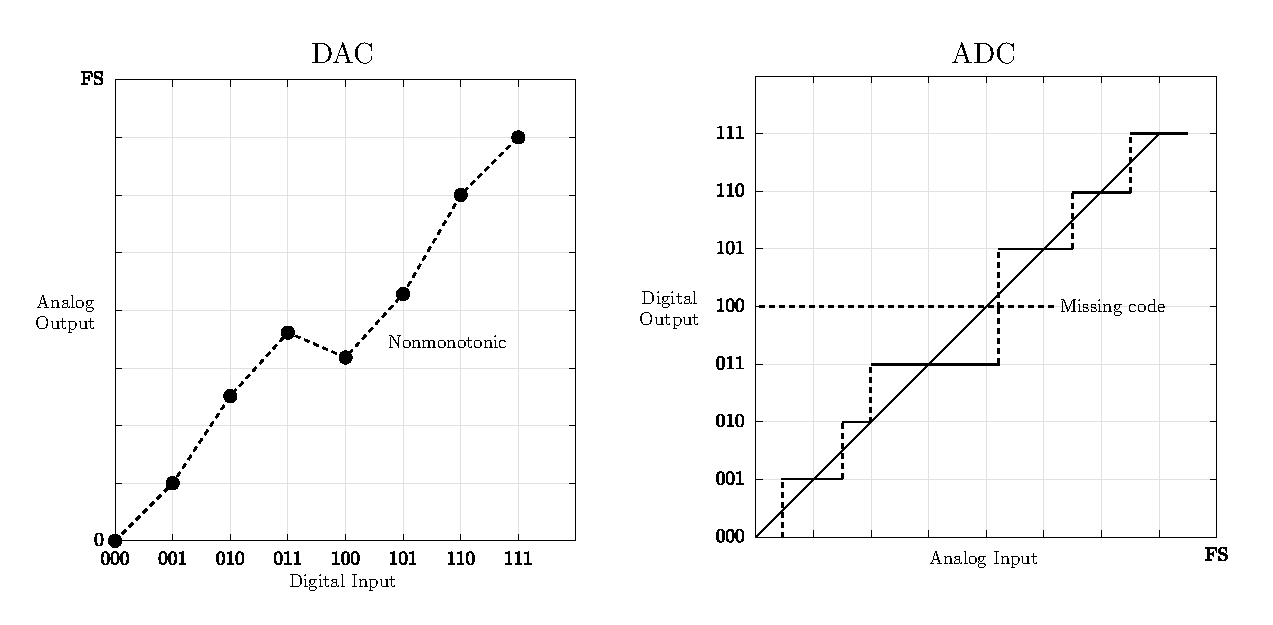
\includegraphics[width=0.95\textwidth]{funcion_de_transferencia_no_ideal}
      \caption{Funciones de transferencia para DAC y ADC no ideales de 3 bits.}
      \label{fig:funcion_de_transferencia_no_ideal}
    \end{figure}

    La monotonía de un DAC a menudo se especifica de manera explícita en las hojas de datos, aunque si se garantiza que el DNL es menor a 1 LSB (es decir, |DNL| $\leq$ 1 LSB ), el dispositivo será monótono, incluso sin una garantía explícita.

    Los ADCs pueden presentar no monotonía, pero un resultado más común del exceso de DNL en los ADCs es la aparición de códigos faltantes. La ausencia de códigos en un ADC es tan problemática como la no monotonía en un DAC. Esto ocurre, al igual que en los DACs, cuando el DNL es inferior a –1 LSB.

    En un DAC, no puede haber códigos faltantes, ya que cada palabra de entrada digital producirá una salida analógica correspondiente. Sin embargo, los DACs pueden ser no monótonos, como se mencionó anteriormente. En un DAC binario directo, el punto más probable para que ocurra una condición de no monotonía es en la mitad de la escala, entre los códigos 011...11 y 100...00. Si se produce una condición de no monotonía en este punto, generalmente se debe a que el DAC no está calibrado o ajustado correctamente. Un ADC de aproximación sucesiva con un DAC interno no monótono normalmente generará códigos faltantes, pero seguirá siendo monótono. Sin embargo, es posible que un ADC sea no monótono, dependiendo de la arquitectura de conversión específica.

   
    %\subsection{Especificaciones generales de un convertidor}


  \subsection{Convertidores Analógico-Digitales}


Las arquitecturas de Conversores Analógico-Digital (ADC) juegan un papel fundamental en la digitalización de señales analógicas, permitiendo la conversión de señales continuas en una representación discreta para su posterior procesamiento digital. En esta sección, se presentan las principales arquitecturas de ADC, incluyendo sus ventajas, desventajas y aplicaciones más comunes. Posteriormente, se realizará una comparación detallada entre estas arquitecturas.


\subsubsection{Convertidor Flash}

El convertidor Flash es la arquitectura de ADC más rápida disponible en la actualidad, ya que realiza la conversión en un solo ciclo. Este tipo de convertidor utiliza $2^{N}-1$ comparadores para realizar la conversión directa de una señal analógica en un código digital de N bits. Cada comparador está polarizado con un valor de referencia que representa una fracción del rango completo de la señal analógica, típicamente espaciada en pasos de un bit menos significativo (LSB). En el caso de un convertidor Flash de 4 bits, la señal analógica se compara simultáneamente con 15 valores de referencia mediante 15 comparadores.

Una de las principales ventajas de los ADC Flash es su alta velocidad, ya que la conversión se lleva a cabo en un solo ciclo. Esto los convierte en la elección preferida para aplicaciones de alta velocidad, como en sistemas de comunicaciones y en aplicaciones de captura de imágenes  donde el tiempo de conversión es crucial. Sin embargo, la desventaja más significativa de los ADC Flash es la cantidad exponencial de comparadores necesarios para aumentar la resolución. Por ejemplo, un ADC de 8 bits requiere 255 comparadores, mientras que uno de 16 bits necesitaría 65,535 comparadores, lo que hace que esta arquitectura sea poco práctica para resoluciones más altas debido a la complejidad del diseño, el alto consumo de energía y el coste.

\subsubsection{Convertidor Pipeline}

El convertidor Pipeline (o de etapas en cascada) resuelve algunas de las limitaciones del ADC Flash, dividiendo el proceso de conversión en varias etapas secuenciales. Cada una de estas etapas incluye un circuito de retención y muestreo, un ADC de $m$ bits (generalmente de tipo Flash), un DAC de $m$ bits. Primero, el circuito de muestreo y retención de la primera etapa adquiere la señal. Luego, el convertidor flash de m bits convierte la señal muestreada en datos digitales. El resultado de la conversión forma los bits más significativos de la salida digital. Esta misma salida digital se introduce en un convertidor digital-analógico de $m$ bits, y su salida se resta de la señal original muestreada. La señal analógica residual se amplifica y se envía a la siguiente etapa de la cadena para ser muestreada y convertida de manera similar a la primera etapa. Este proceso se repite en tantas etapas como sean necesarias para lograr la resolución deseada. En principio, un convertidor en pipeline con $p$ etapas, cada una con un convertidor flash de $m$ bits, puede producir un ADC de alta velocidad con una resolución de $R = p \times m $ bits, utilizando $p \times (2^m - 1)$ comparadores.

Una ventaja clave de los ADCs Pipeline es que permiten obtener resoluciones más altas que los ADCs Flash sin requerir un número exponencial de comparadores. Por ejemplo, un ADC de Pipeline con dos etapas de 8 bits requiere solo 30 comparadores en lugar de los 255 que necesitaría un ADC Flash de 8 bits. Además, los convertidores Pipeline pueden alcanzar tasas de conversión comparables a los ADCs Flash, ya que las etapas posteriores pueden procesarse de manera simultánea con diferentes señales, maximizando el rendimiento. Sin embargo, una desventaja de los ADC Pipeline es la latencia igual a $p$ ciclos introducida por las múltiples etapas, lo que los hace menos adecuados para aplicaciones que requieren una conversión inmediata.


\subsubsection{Convertidor de Aproximaciones Sucesivas (SAR)}

El convertidor de Aproximaciones Sucesivas (SAR) sigue un principio de funcionamiento diferente al del ADC Flash. En lugar de realizar todas las comparaciones de manera simultánea, el ADC SAR emplea un único comparador que realiza una serie de comparaciones secuenciales. El proceso comienza comparando la señal analógica con la mitad de la escala completa (correspondiente al bit más significativo) y, en función del resultado, retiene o descarta ese valor. El proceso se repite para los siguientes bits de menor peso, reduciendo progresivamente el rango de comparación hasta alcanzar la resolución deseada.

La arquitectura SAR es eficiente en términos de hardware, ya que requiere solo un comparador y un DAC de alta precisión para generar los niveles de referencia. Sin embargo, debido a que el ADC SAR necesita $N$ ciclos de comparación para resolver una conversión de $N$ bits, su velocidad es inferior a la de los ADCs Flash y Pipeline. A pesar de ello, el ADC SAR es ideal para aplicaciones de alta resolución y baja velocidad, como la adquisición de señales no periódicas o señales que requieren alta precisión, como en la instrumentación médica. Además, el ADC SAR es altamente eficiente en términos de consumo de energía y es una opción común en aplicaciones de bajo consumo.


\subsubsection{Convertidor Sigma-Delta}

El convertidor Sigma-Delta ($\Sigma \Delta$) emplea un enfoque completamente diferente al de las arquitecturas anteriores. En lugar de realizar una conversión directa de la señal analógica en un número binario, el ADC Sigma-Delta sobreamuestrea la señal analógica y la convierte en una secuencia de bits a través de un proceso de integración y comparación. Este flujo de bits se procesa mediante un filtro digital y se decima para obtener una salida digital de alta resolución.

El Sigma-Delta es la arquitectura preferida para aplicaciones que requieren alta resolución y bajo ancho de banda, como la medición de precisión en instrumentos científicos. Una de las principales ventajas del ADC Sigma-Delta es su capacidad para mitigar el ruido de baja frecuencia mediante el modelado de ruido, desplazando gran parte de ese ruido a frecuencias más altas, fuera de la banda de interés. Además, debido al alto índice de sobremuestreo, la necesidad de filtros anti-alias externos se reduce significativamente. Sin embargo, una de las limitaciones del ADC Sigma-Delta es su alta latencia, lo que lo hace inadecuado para aplicaciones de respuesta rápida o señales multiplexadas.

\subsubsection{Comparación entre las Arquitecturas de ADC}

En la Tabla \ref{tab:adcs_comparacion} se presenta una comparación detallada entre las principales arquitecturas de ADC en función de parámetros clave como la velocidad, resolución, latencia, complejidad de diseño y adecuación para aplicaciones específicas.

 \begin{table}[h!]
      \caption{Comparación entre arquitecturas de ADC.}
      \begin{center}
      \resizebox{\textwidth}{!}{
        \begin{NiceTabular}{|c|c|c|c|c|c|}
       \hline
        \textbf{Arquitectura} & \textbf{Velocidad} & \textbf{Resolución} & \textbf{Latencia} & \textbf{Complejidad} & \textbf{Aplicación Ideal} \\
        \hline
        Flash & Muy alta & Baja & Muy baja & Muy alta & Sistemas de alta velocidad (telecomunicaciones) \\
        Pipeline & Alta & Media-alta & Media & Alta & Alta resolución con alta velocidad (imagen, radar) \\
        SAR & Media & Alta & Baja & Baja & Instrumentación de precisión, adquisición de datos \\
        Sigma-Delta & Baja & Muy alta & Alta & Media-alta & Medición de precisión, instrumentos científicos \\
        \hline
        \end{NiceTabular}
      }
      \label{tab:adcs_comparacion}
      \end{center}
    \end{table}

La Tabla \ref{tab:adc_resumen} resume y clasifica (de manera general) las ventajas relativas de las arquitecturas flash, pipeline, SAR y sigma-delta. Una clasificación de 1 en una categoría de rendimiento indica que la arquitectura es inherentemente superior a las demás en esa categoría. Un * indica que la arquitectura posee la capacidad o característica mencionada.

 \begin{table}[h!]
      \caption{Resumen de tipos de ADC.}
      \begin{center}
      \resizebox{\textwidth}{!}{
        \begin{NiceTabular}{|c|c|c|c|c|}
          \hline
          \textbf{Características} & \textbf{Flash} & \textbf{Pipelined} & \textbf{SAR} & \textbf{Sigma-Delta}\\ 
          \hline
           Rendimiento & 1 & 2 & 3 & 4 \\ 
           Resolución  & 4 & 3 & 2 & 1 \\ 
           Latencia & 1 & 3 & 2 & 4 \\ 
           Adecuación para convertir múltiples señales por ADC & 1 & 2 & 1 & 3 \\ 
           Capacidad para convertir señales multiplexadas no periódicas & 1 & 2 & 1 & 3 \\ 
           Antialiasing simplificado &  &  &  & $\star$ \\ 
           Puede realizar submuestreo & $\star$ & $\star$ & $\star$ &  \\ 
           Puede aumentar la resolución mediante promediado (con ruido de trémulo) & $\star$ & $\star$ & $\star$ &  \\
          \hline
        \end{NiceTabular}
      }
      \label{tab:adc_resumen}
      \end{center}
    \end{table}

La elección de la arquitectura adecuada depende en gran medida de los requisitos específicos de la aplicación. Por ejemplo, en aplicaciones donde se requiere una alta tasa de muestreo, como en comunicaciones o adquisición de imágenes, los convertidores Flash o Pipeline son ideales debido a su alta velocidad de conversión. Por otro lado, si se necesita alta resolución con señales de bajo ancho de banda, como en la instrumentación de precisión, los convertidores Sigma-Delta son la opción más adecuada. Los convertidores SAR, por su parte, son ideales para aplicaciones que requieren alta precisión con un coste relativamente bajo y bajo consumo de energía.


